\documentclass[14pt]{extarticle}
\usepackage{fontspec}
\usepackage{polyglossia}
\usepackage{amsmath}
\usepackage{amssymb}
\usepackage{xcolor}
\usepackage{fancyhdr}
\usepackage{graphicx}
\usepackage{listings}
\usepackage[most]{tcolorbox}
% \usepackage{setspace}
\usepackage{pifont}
\usepackage{enumitem}
\usepackage{titlesec}
\usepackage[bottom]{footmisc}
\usepackage{titling}
\usepackage{minted}
\usepackage{etoolbox}
\usepackage{array}
\usepackage{extsizes}
\usepackage{float}
\usepackage{booktabs}
\usepackage{hyperref}
\usepackage[onehalfspacing]{setspace}
\usepackage[a4paper, top=2.7cm, bottom=2.7cm, left=2.5cm, right=2.5cm, headheight=1.5cm, headsep=0.5cm]{geometry}
\usepackage{tikz}

\usetikzlibrary{automata, positioning, arrows.meta, arrows}

\newfontfamily\emoji{Segoe UI Emoji}

\pagestyle{fancy}

\setmainlanguage[numerals=western]{arabic}
\setotherlanguage{english}
% \newfontfamily\arabicfont[Script=Arabic]{Amiri}
\newfontfamily\arabicfont[Script=Arabic]{Calibri}
\newfontfamily\arabicfonttt[Script=Arabic]{Courier New}

\lstset{
  language=[Sharp]C,
  numbers=left,
  stepnumber=1,
  numbersep=8pt,
  frame=single,
  basicstyle=\ttfamily\small,
  keywordstyle=\color{blue},
  stringstyle=\color{red},
  commentstyle=\color{green!50!black}
}

\newif\ifdetailed
\ifdefined\setdetailed
  \setdetailed
\fi

\newif\ifwithsols
\ifdefined\setwithsols
  \setwithsols
\fi

% unified tcolorboxes for articles
\tcbset{colback=white, colframe=black, fonttitle=\bfseries, boxrule=0.8pt}
\newtcolorbox{boxDef}[1][]{colback=blue!5!white,colframe=blue!75!black,
  title={{\emoji📘} تعريف\ifx\\#1\\\else ~#1\fi :}}
\newtcolorbox{boxExercise}[1][]{colback=cyan!5!white,colframe=cyan!70!black,
  title={{\emoji🧩} تمرين\ifx\\#1\\\else ~#1\fi :}}
\newtcolorbox{boxExample}[1][]{colback=yellow!5!white,colframe=orange!90!black,
  title={{\emoji📝} مثال\ifx\\#1\\\else ~#1\fi :}}
\newtcolorbox{boxNote}[1][]{colback=gray!10!white,colframe=black,
  title={{\emoji✨} ملاحظة\ifx\\#1\\\else ~#1\fi :}}
\newtcolorbox{boxAttention}[1][]{colback=magenta!10!white,colframe=magenta!80!black,
  title={{\emoji🔔} تنبيه\ifx\\#1\\\else ~#1\fi :}}
\newtcolorbox{boxWarning}[1][]{colback=red!5!white,colframe=red!75!black,
  title={{\emoji⚡} ملاحظة هامة\ifx\\#1\\\else ~#1\fi :}}
\newtcolorbox{boxSolution}[1][]{colback=green!5!white,colframe=green!60!black,
  title={{\emoji✅} حل\ifx\\#1\\\else ~#1\fi :}}
\newtcolorbox{boxSymbol}[1][]{colback=purple!5!white,colframe=purple!70!black,
  title={{\emoji🔣} رمز\ifx\\#1\\\else ~#1\fi :}}
\newtcolorbox{boxHint}[1][]{colback=teal!5!white,colframe=teal!60!black,
  title={{\emoji💡} تلميح\ifx\\#1\\\else ~#1\fi :}}


\tcbset{simplecode/.style={ colback=gray!5, colframe=black!50, boxrule=0.4pt, arc=2pt, left=4pt,right=4pt,top=4pt,bottom=4pt}}
\newenvironment{boxCode}{\begin{tcolorbox}[simplecode]}{\end{tcolorbox}}

\newcolumntype{C}[1]{>{\centering\arraybackslash}p{#1}}

% redefine spaces after titles
\makeatletter
\renewcommand{\@maketitle}{%
  \begin{center}
    {\huge \bfseries \@title \par}%
    \vskip 0.2em % space between title and author
    {\large \@author \par}%
    % \vskip 0.2em % space between author and date
    % {\normalsize \@date \par}%
  \end{center}
}
\makeatother

\fancyhf{} % clear default
\fancypagestyle{plain}{
  \fancyhf{}
  \fancyhead[L]{مدرسة التسامح الشاملة}
  % \fancyhead[L]{
\includegraphics[height=1cm]{../../../images/logoTasamoh.png}}
  \fancyhead[R]{الأستاذ محمود اغبارية}
  \fancyfoot[C]{\thepage}
}

\fancyhead[L]{مدرسة التسامح الشاملة}
\fancyhead[R]{الأستاذ محمود اغبارية}
\fancyfoot[C]{\thepage}
% \date{\today}

\setcounter{tocdepth}{3} % only section subsection and subsubsection in TOC

\newcommand{\importpdfpage}[2]{%
    \thispagestyle{empty}
    \newgeometry{left=0cm,right=0cm,top=0cm,bottom=0cm}
    \includegraphics[page=#2,width=0.95\paperwidth,height=0.95\paperheight,keepaspectratio]{#1}
    \restoregeometry
}

\newcommand{\insertFullImg}[1]{%
    \noindent
    \makebox[\textwidth][c]{
        \includegraphics[width=0.9\paperwidth,keepaspectratio]{#1}%
    }%
}%

% ----------------------


% \begin{document}

% \maketitle

% % \clearpage  % start TOC on a new page
% % \renewcommand{\contentsname}{جدول المحتويات}
% % \tableofcontents
% % \clearpage

% \part*{part 1} % the * prevents numbering
% \section*{مقدمة}
% \subsection*{مثال رياضي}
% \subsubsection*{مثال فرعي}
% \paragraph*{ paragraph 1}
% \subparagraph*{sub paragraph 1}

% \ifdetailed
% \begin{english}
% \begin{minted}{csharp}
% // C# Example
% \end{minted}
% \end{english}
% \fi

% OLD WAY
% \ifdetailed
% \begin{english}
% \begin{lstlisting}
% // C# Example
% \end{lstlisting}
% \end{english}
% \fi

% % 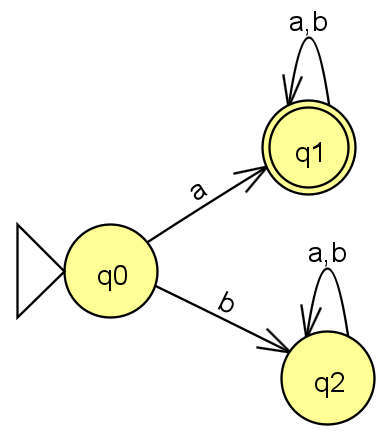
\includegraphics[width=0.2\textwidth]{../../../images/DFAs/ex1_q1.png}



% \vspace{3cm}
% \begin{flushleft}
% أرجو لكم وقتًا ممتعًا.

% الأستاذ محمود اغبارية.
% \end{flushleft}


% \end{document}


\ifwithsols
\title{حل وظيفة عطلة الربيع \\ أسئلة بجروت عن المصفوفات}
\else
\title{وظيفة عطلة الربيع \\ أسئلة بجروت عن المصفوفات}
\fi

\begin{document}

\maketitle
\thispagestyle{fancy}


\subsection*{تعليمات}
{\large
\begin{itemize}[itemsep=1em]
    \item يجب حل جميع الأسئلة في هذا الملف.
    \item اكتب عنوان السؤال بشكل واضح (رقم السؤال، والسنة ورقم النموذج.)
    \item يجب كتابة الحلول يدويًّا وليس على الحاسوب، بخطّ واضح ومقروء.
    \item تُسّلَّم الحلول ورقيًّا يوم \textenglish{\textbf{الاثنين 20.5.2026}}
    \item \textbf{الحل النهائي المكتوب في الورقة التي تسلمها يجب أن يكون حلك بنفسك}، لا مانع قبل ذلك من استخدام مصادر خارجية يشمل زملاء الدراسة والذكاء الاصطناعي. لكن لا تنسخ منهم، افهم ثم اكتب الحل كاملًا بنفسك.
    \item الحل المنسوخ عن طالب آخر أو عن الذكاء الاصطناعي سيحصل على علامة 0.
    \item حل هذه الأسئلة وتسليمها يشكل $20\%$ من العلامة النهائية للفصل الثالث.
\end{itemize}
}

\vspace{1cm}
\begin{flushleft}
أرجو لكم عملا ممتعًا وعطلة ناجعة.

الأستاذ محمود اغبارية.
\end{flushleft}

\ifwithsols
\else
\clearpage
\fi

\subsection*{سؤال 1 امتحان 899381a سنة 2020}
\addcontentsline{toc}{subsection}{سؤال 1 امتحان 899381a سنة 2020}

\noindent
\makebox[\textwidth][c]{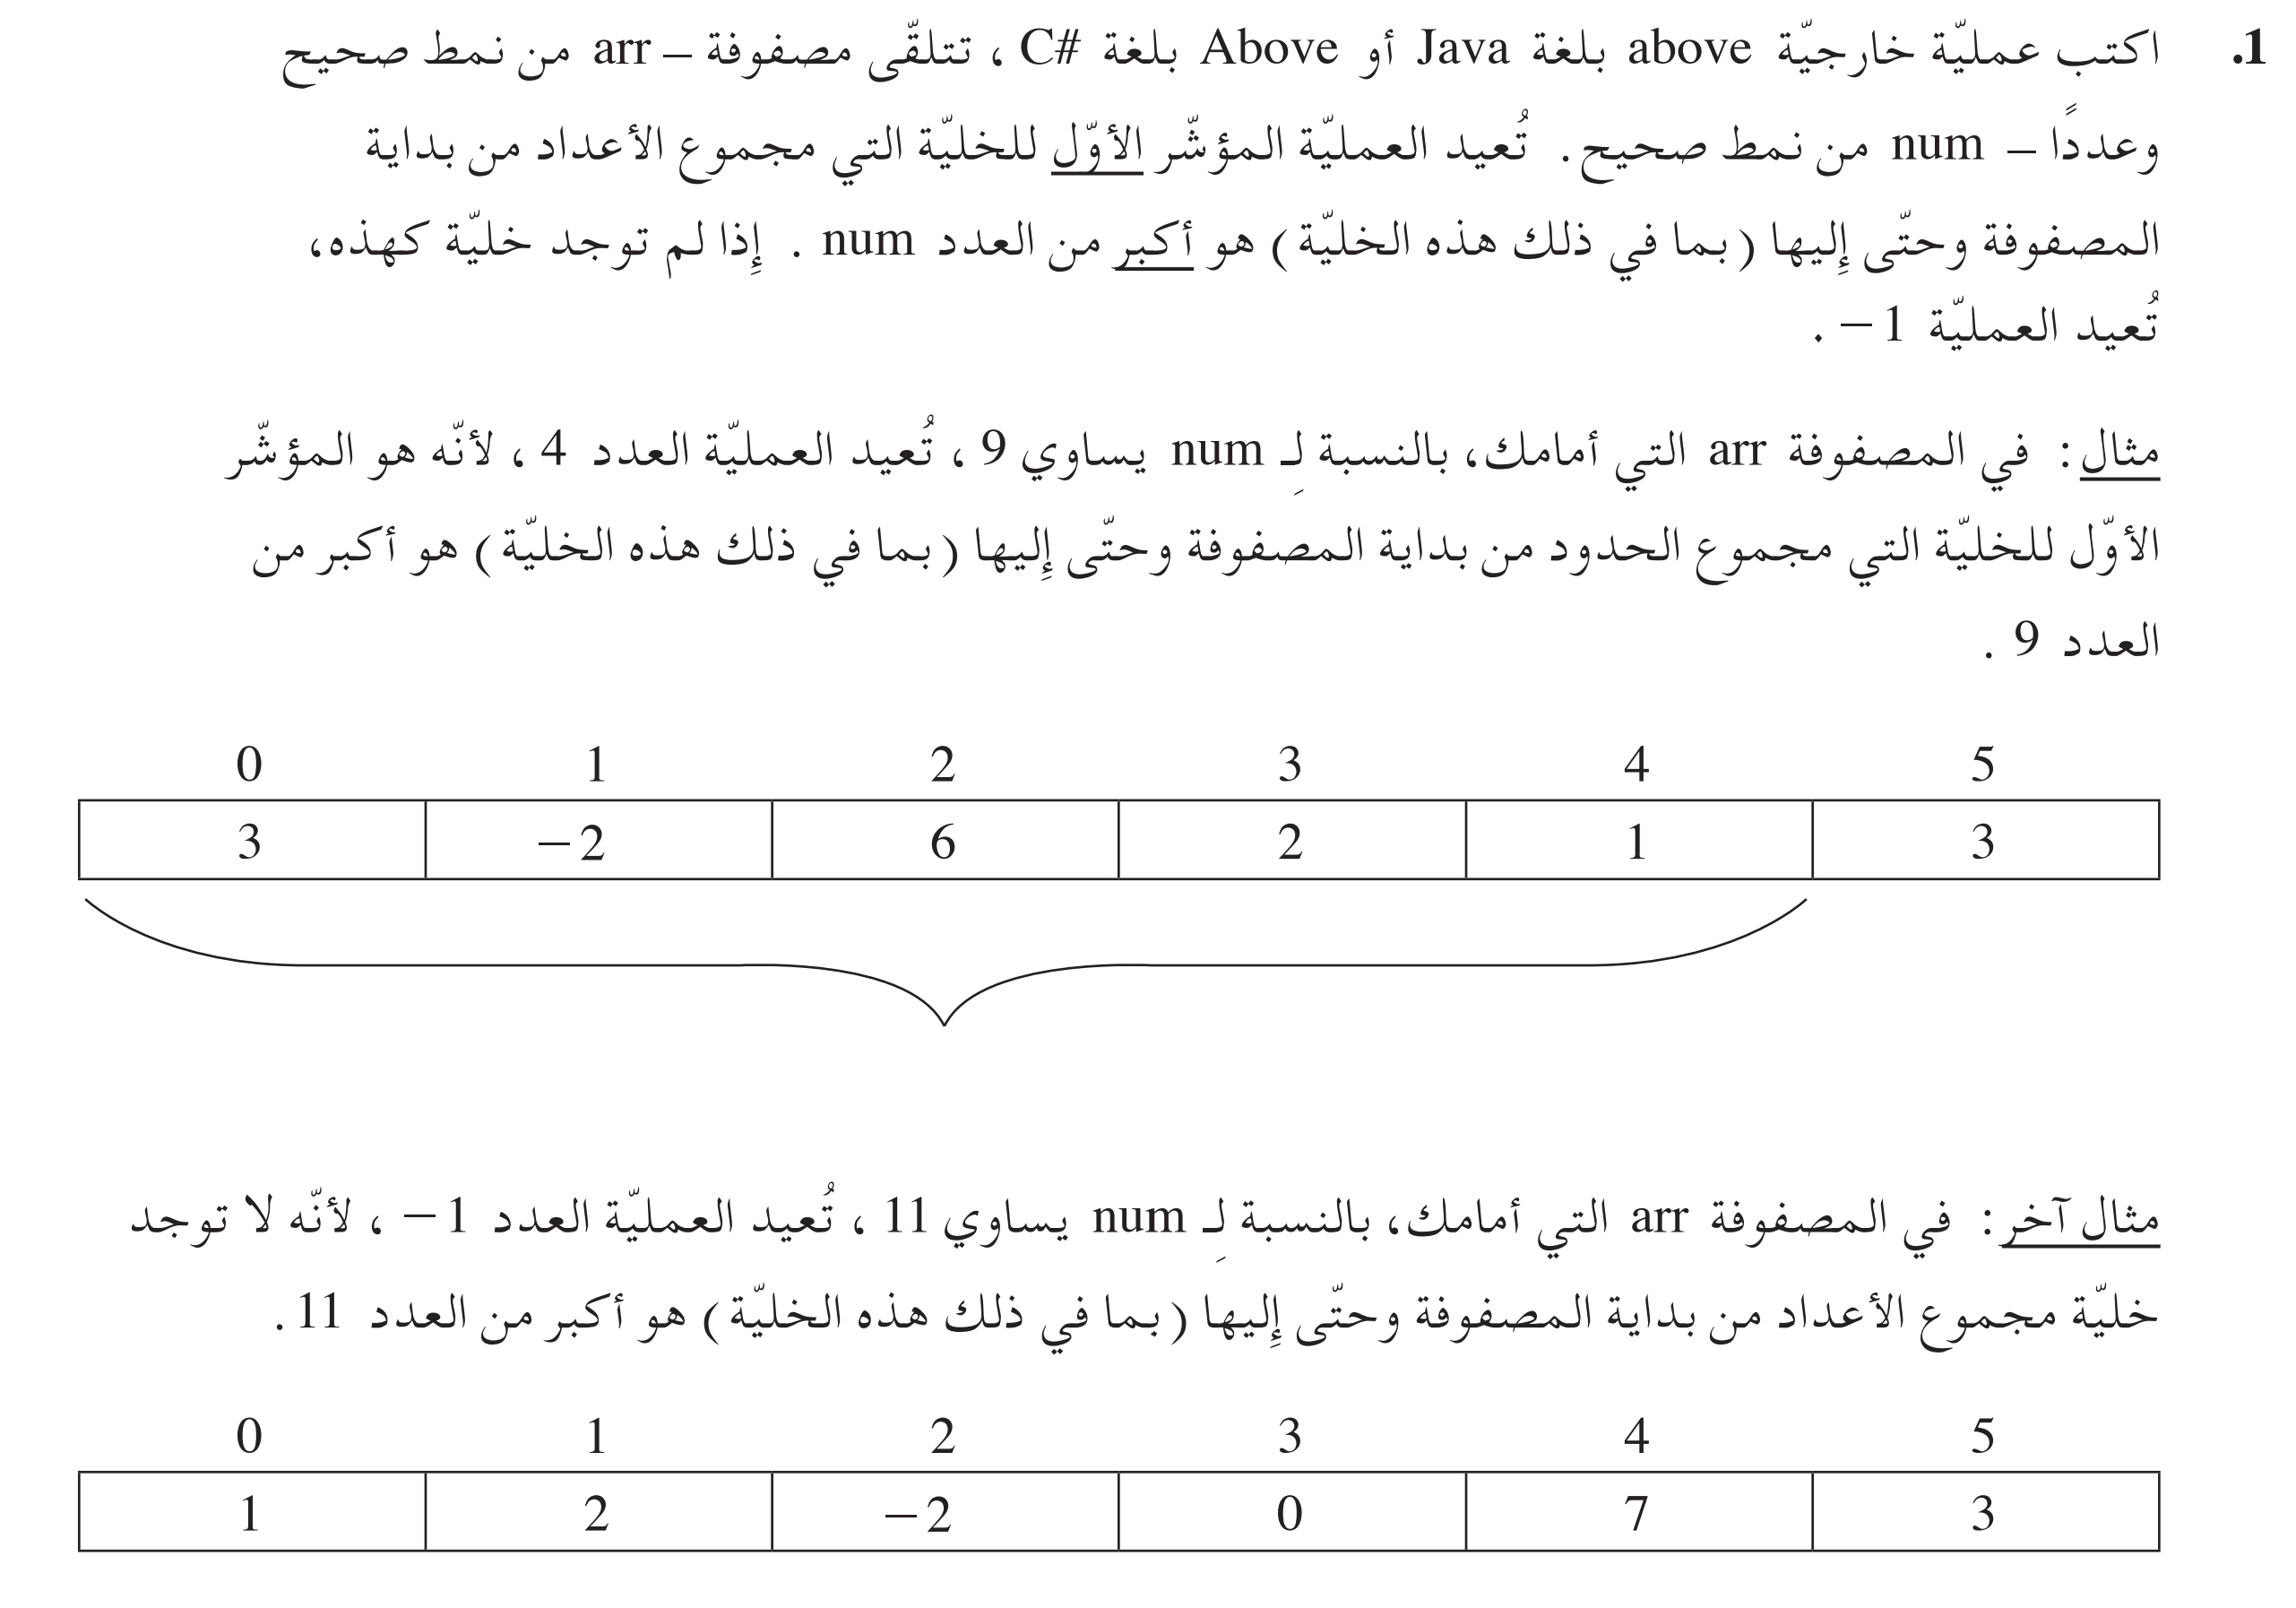
\includegraphics[width=0.9\paperwidth,keepaspectratio]{ ../../../bagrut_questions/basics/arrays_2020_899381a_1.png }%
}%

\ifwithsols
\begin{boxSolution}[سؤال 1 امتحان 899381a سنة 2020]

\begin{boxCode}
\begin{english}
\begin{minted}{csharp}
public static int Above(int[] arr, int num)
{
    int sum = 0;
    for (int i = 0; i < arr.Length; i++)
    {
        sum += arr[i];
        if (sum > num)
            return i;
    }
    return -1;
}
\end{minted}
\end{english}
\end{boxCode}

\end{boxSolution}
\clearpage
\fi

\ifwithsols
\else
\clearpage
\fi

\subsection*{سؤال 1 امتحان 899381a سنة 2021}
\addcontentsline{toc}{subsection}{سؤال 1 امتحان 899381a سنة 2021}

\noindent
\makebox[\textwidth][c]{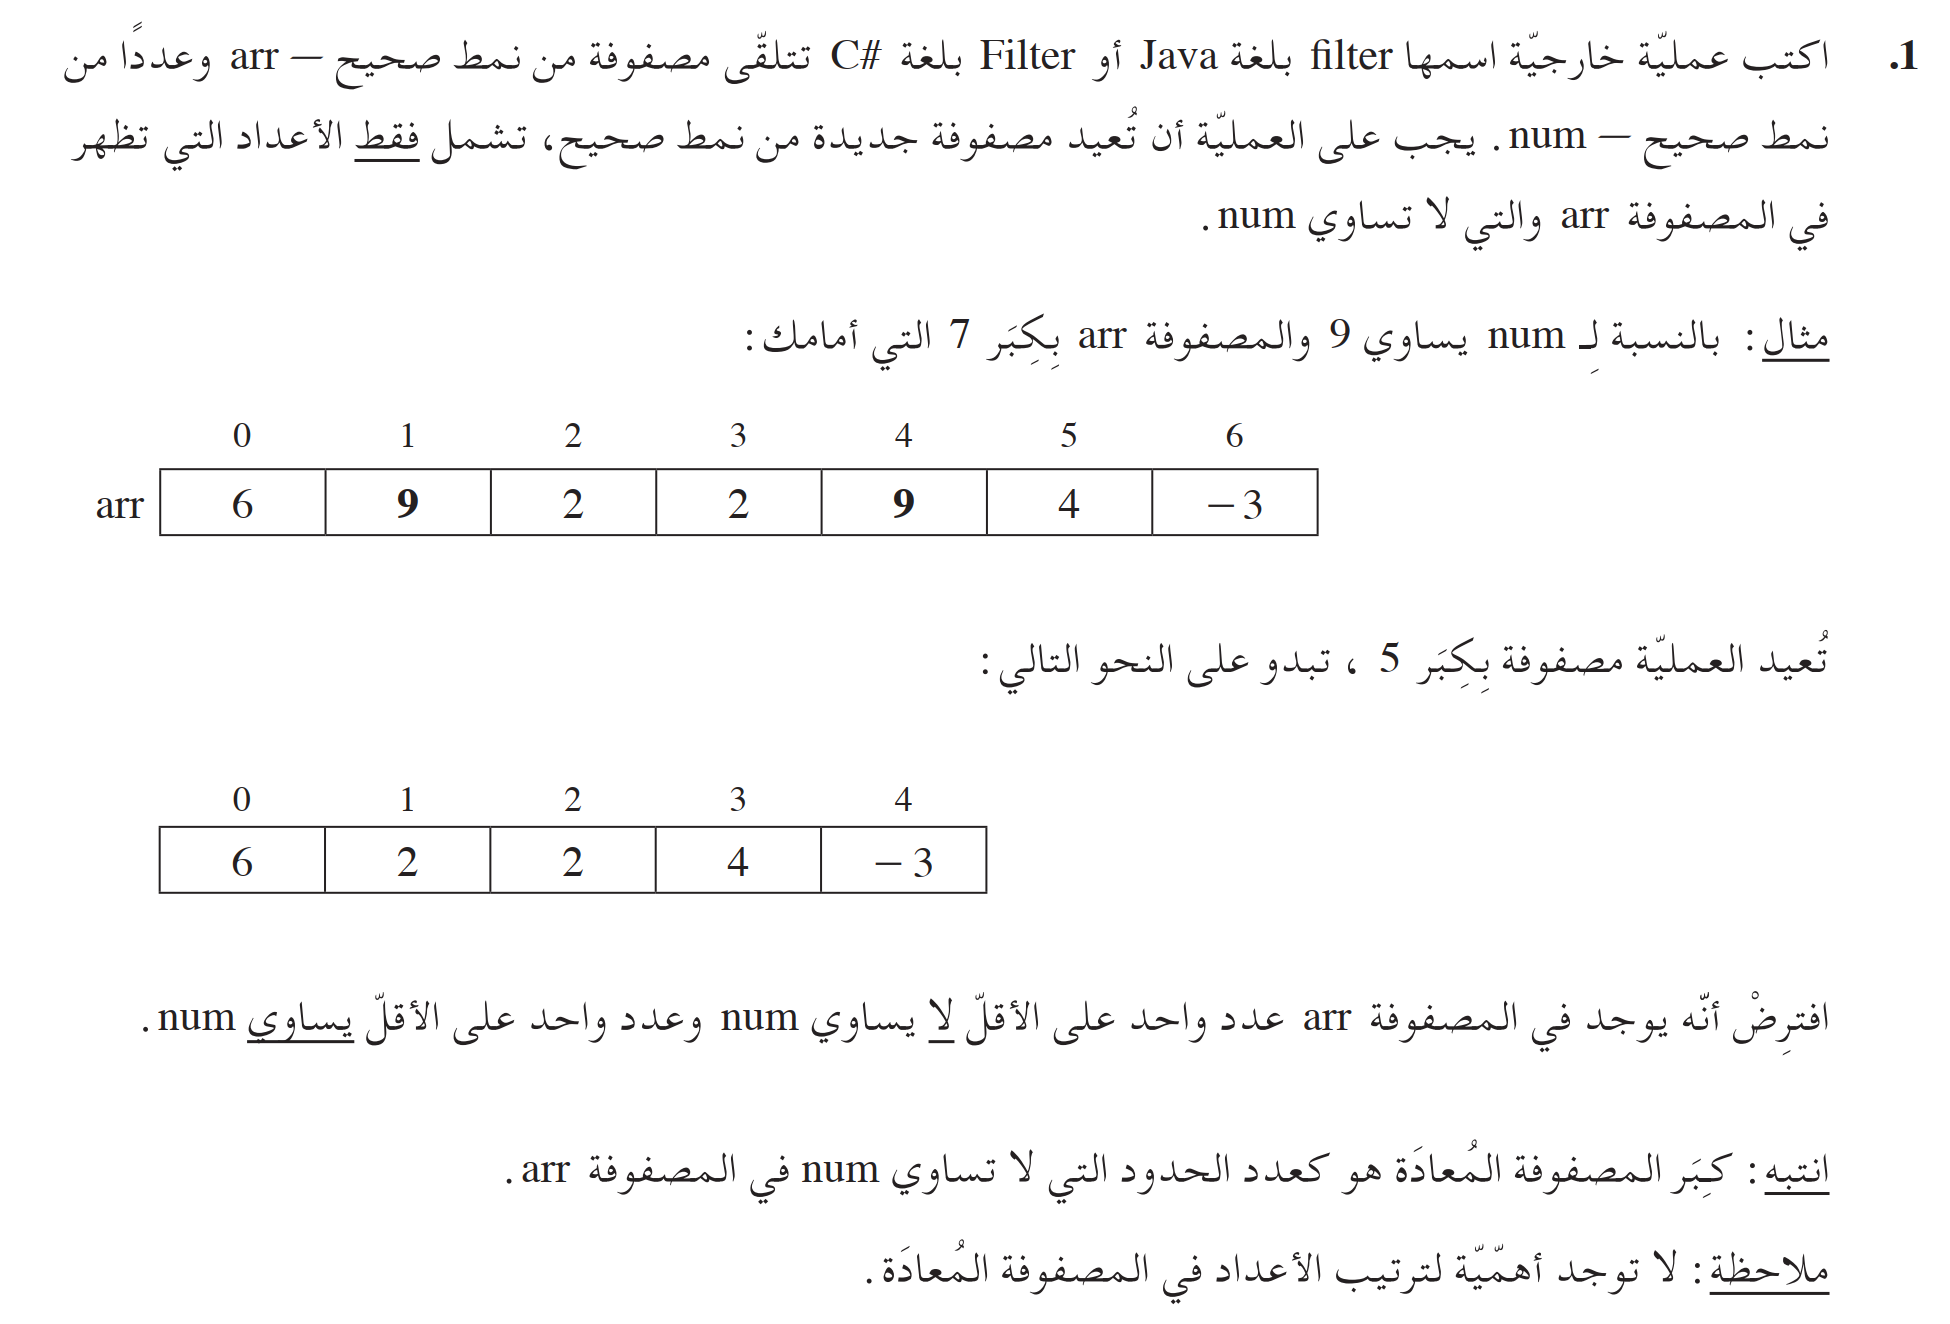
\includegraphics[width=0.9\paperwidth,keepaspectratio]{ ../../../bagrut_questions/basics/arrays_2021_899381a_1.png }%
}%


\ifwithsols
\begin{boxSolution}[سؤال 1 امتحان 899381a سنة 2021]

\begin{boxCode}
\begin{english}
\begin{minted}{csharp}
public static int[] Filter(int[] arr, int num)
{
    int count = 0;
    for (int i = 0; i < arr.Length; i++)
    {
        if (arr[i] != num)
            count++;
    }

    int[] result = new int[count];
    int index = 0;
    for (int i = 0; i < arr.Length; i++)
    {
        if (arr[i] != num)
        {
            result[index] = arr[i];
            index++;
        }
    }
    return result;
}
\end{minted}
\end{english}
\end{boxCode}

\end{boxSolution}
\clearpage
\fi

\ifwithsols
\else
\clearpage
\fi

\subsection*{سؤال 1 امتحان 899381 سنة 2022}
\addcontentsline{toc}{subsection}{سؤال 1 امتحان 899381 سنة 2022}

\noindent
\makebox[\textwidth][c]{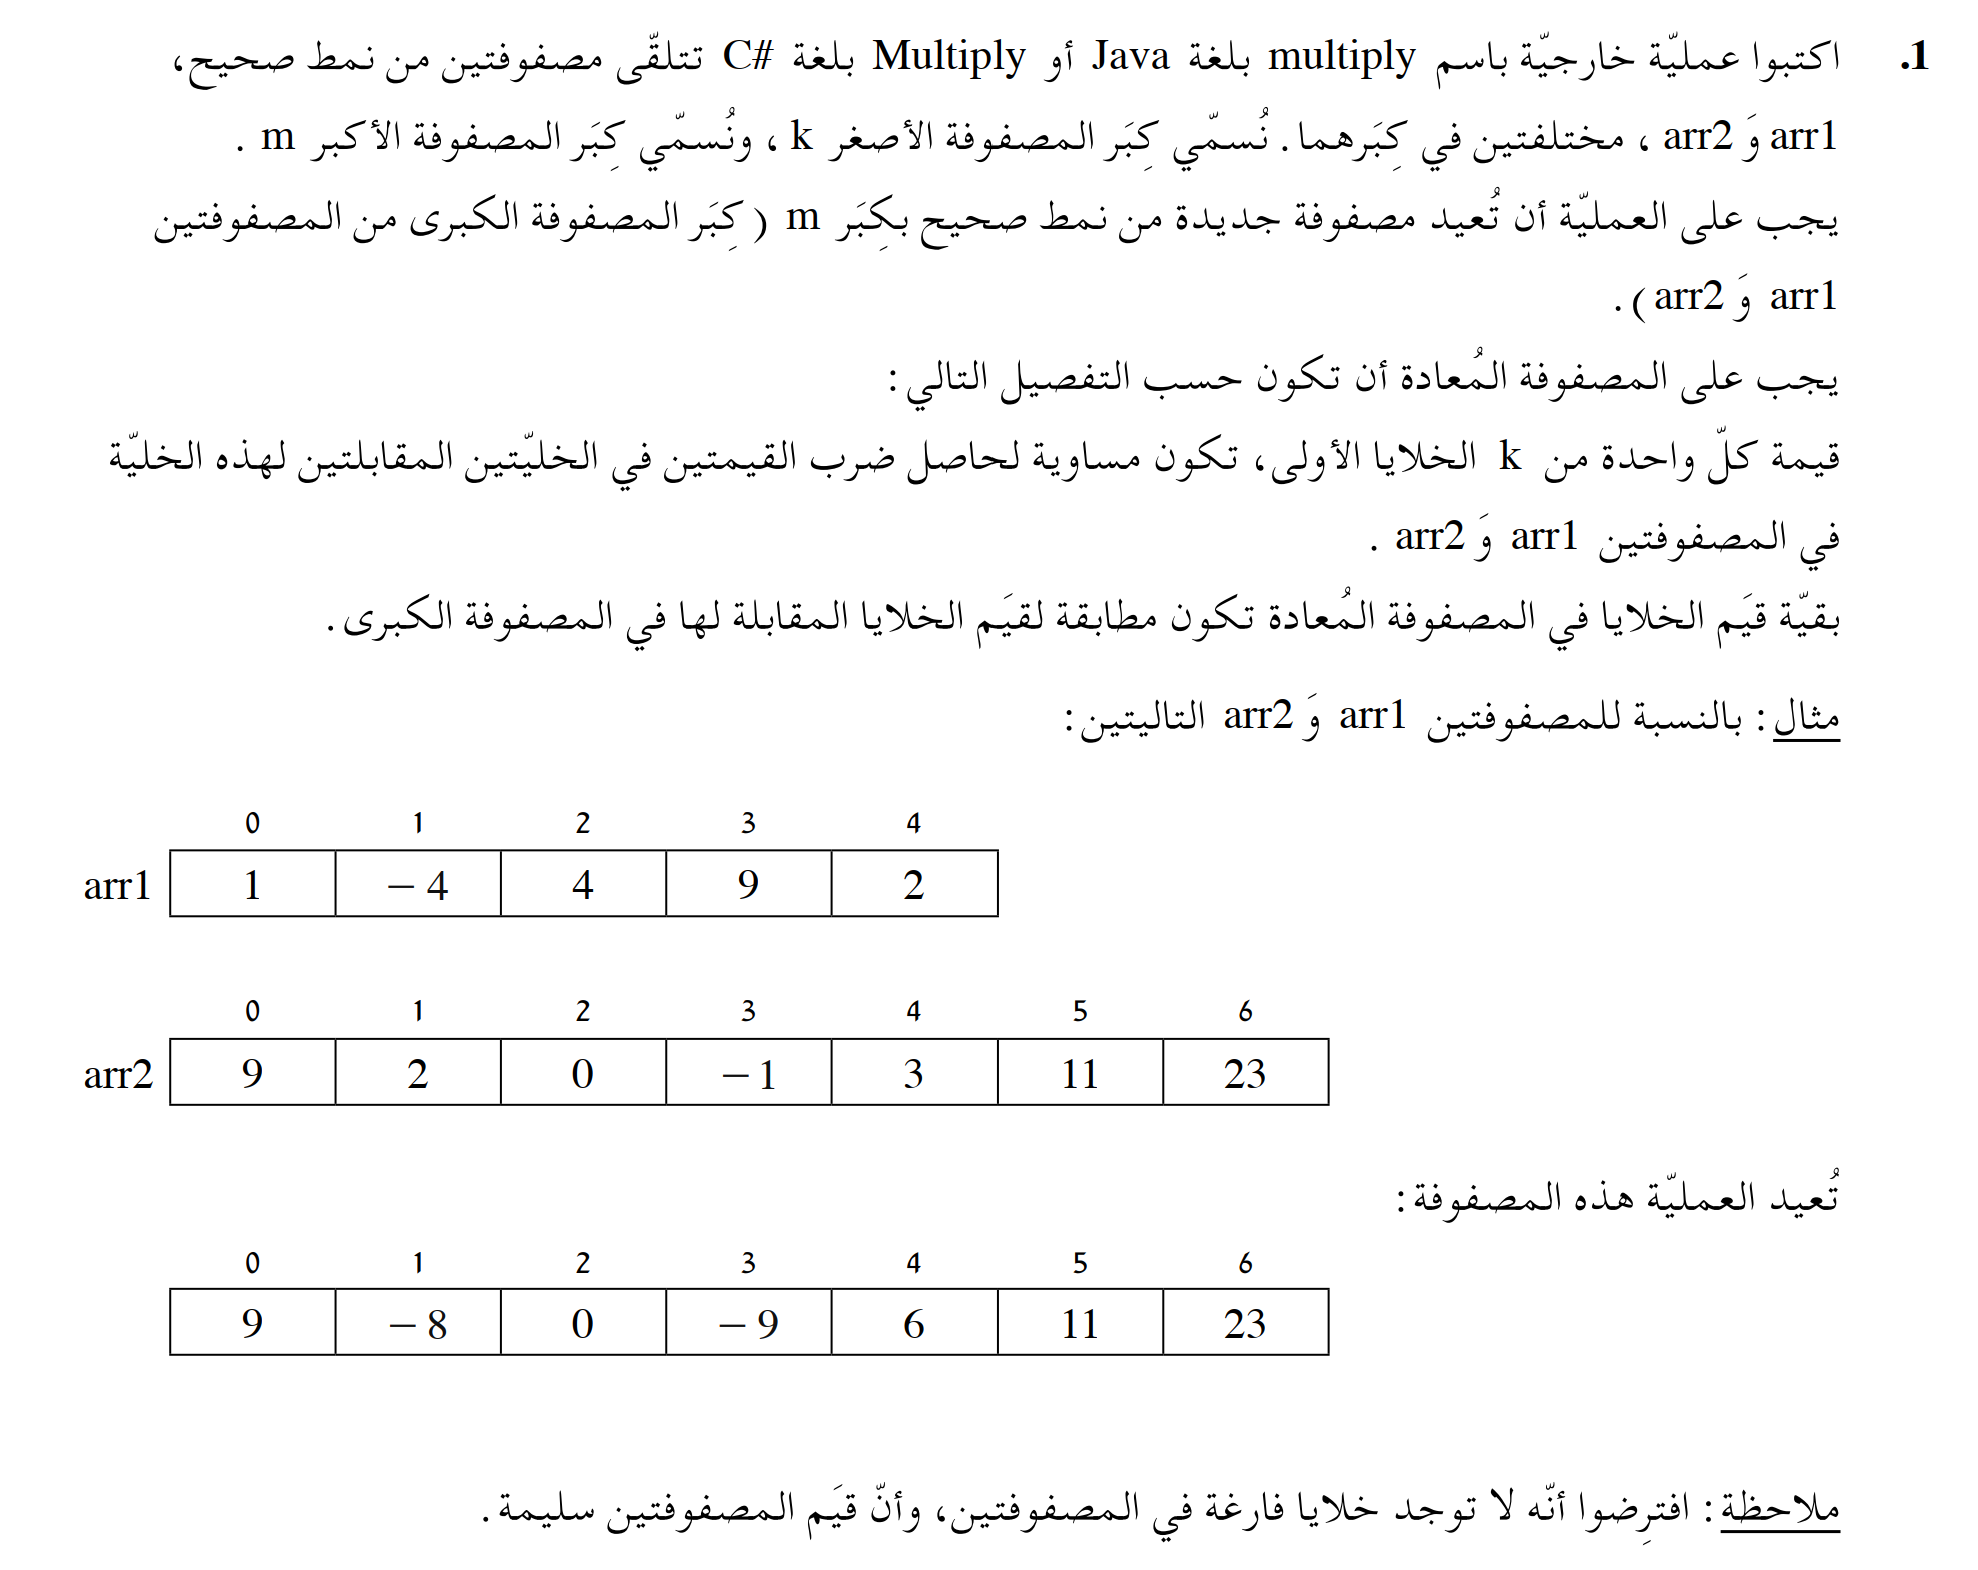
\includegraphics[width=0.9\paperwidth,keepaspectratio]{ ../../../bagrut_questions/basics/arrays_2022_899381_1.png }%
}%


\ifwithsols
\begin{boxSolution}[سؤال 1 امتحان 899381 سنة 2022]

\begin{boxCode}
\begin{english}
\begin{minted}{csharp}
public static int[] Multiply(int[] arr1, int[] arr2)
{
    if(arr1.Length > arr2.Length)
    {
        int[] temp = arr1;
        arr1 = arr2;
        arr2 = temp;
    }
    // now we know arr1 is the shorter array
    int m = arr2.Length;
    int k = arr1.Length;
    int[] result = new int[m];
    for (int i = 0; i < k; i++)
    {
        result[i] = arr1[i] * arr2[i];
    }
    for (int i = k; i < m; i++)
    {
        result[i] = arr2[i];
    }
    return result;
}
\end{minted}
\end{english}
\end{boxCode}

\end{boxSolution}
\clearpage
\fi

\ifwithsols
\else
\clearpage
\fi

\subsection*{سؤال 1 امتحان 899381 سنة 2023}
\addcontentsline{toc}{subsection}{سؤال 1 امتحان 899381 سنة 2023}

\noindent
\makebox[\textwidth][c]{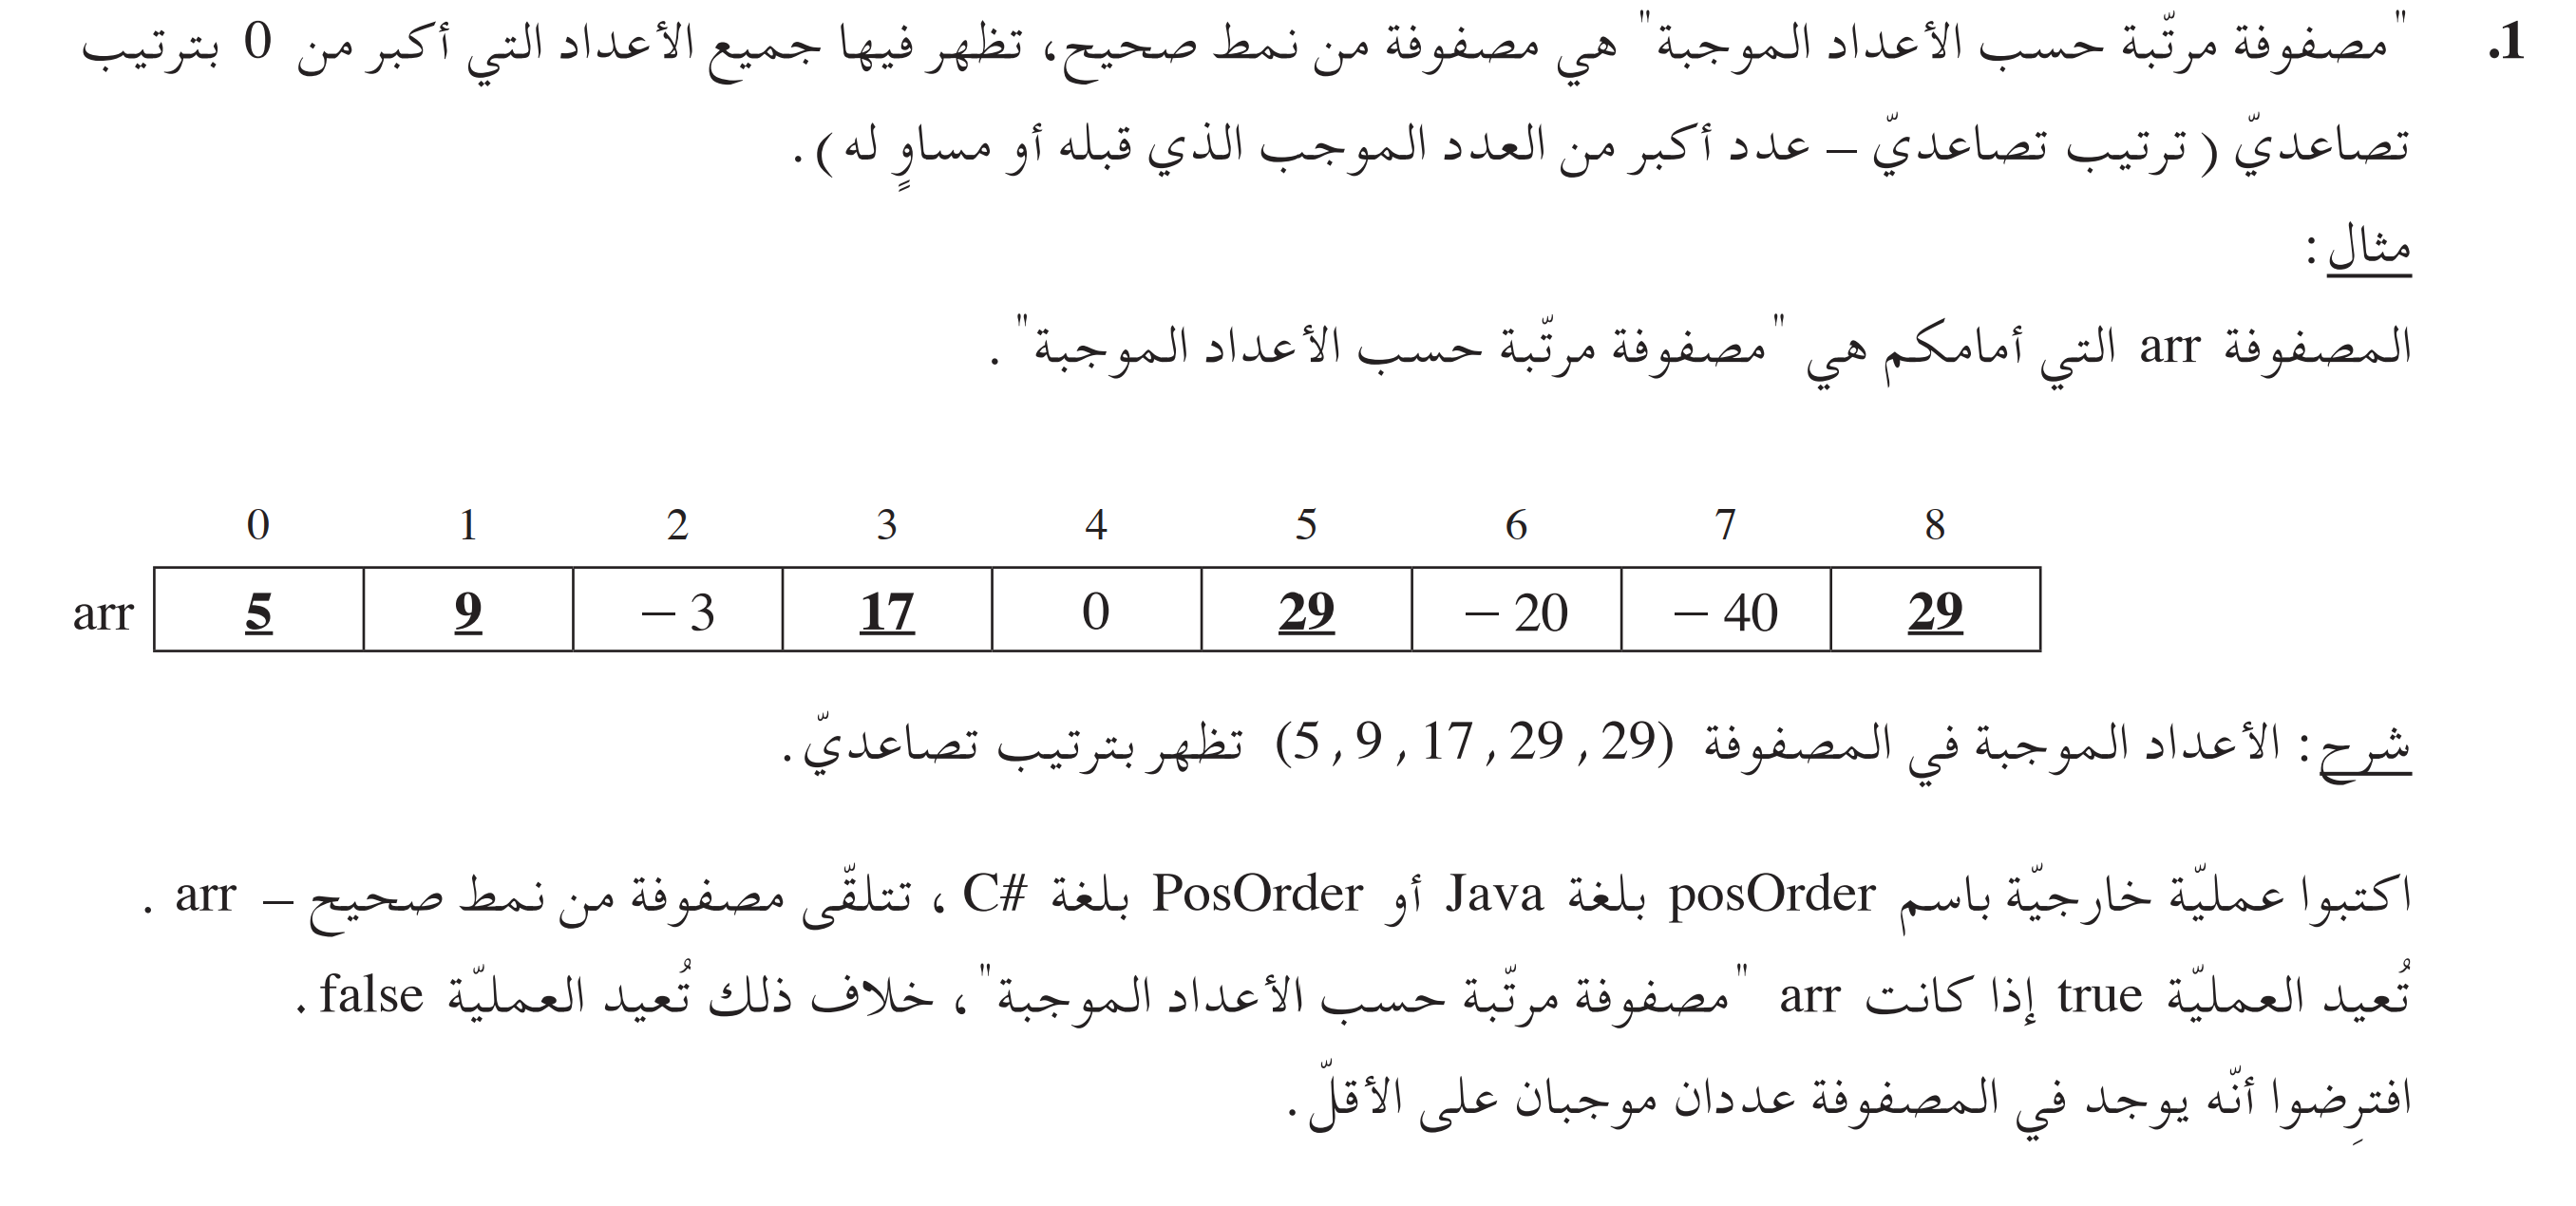
\includegraphics[width=0.9\paperwidth,keepaspectratio]{ ../../../bagrut_questions/basics/arrays_2023_899381_1.png }%
}%


\ifwithsols
\begin{boxSolution}[سؤال 1 امتحان 899381 سنة 2023]
\begin{boxCode}
\begin{english}
\begin{minted}{csharp}
public static bool PosOrder(int[] arr)
{
    int previousPositive = 0;
    for (int i = 0; i < arr.Length; i++)
    {
        if (arr[i] > 0)
        {
            if (arr[i] < previousPositive)
                return false;
            previousPositive = arr[i];
        }
    }
    return true;
}
\end{minted}
\end{english}
\end{boxCode}

\end{boxSolution}
\clearpage
\fi

\ifwithsols
\else
\clearpage
\fi

\subsection*{سؤال 2 امتحان 899381 سنة 2022}
\addcontentsline{toc}{subsection}{سؤال 2 امتحان 899381 سنة 2022}

\noindent
\makebox[\textwidth][c]{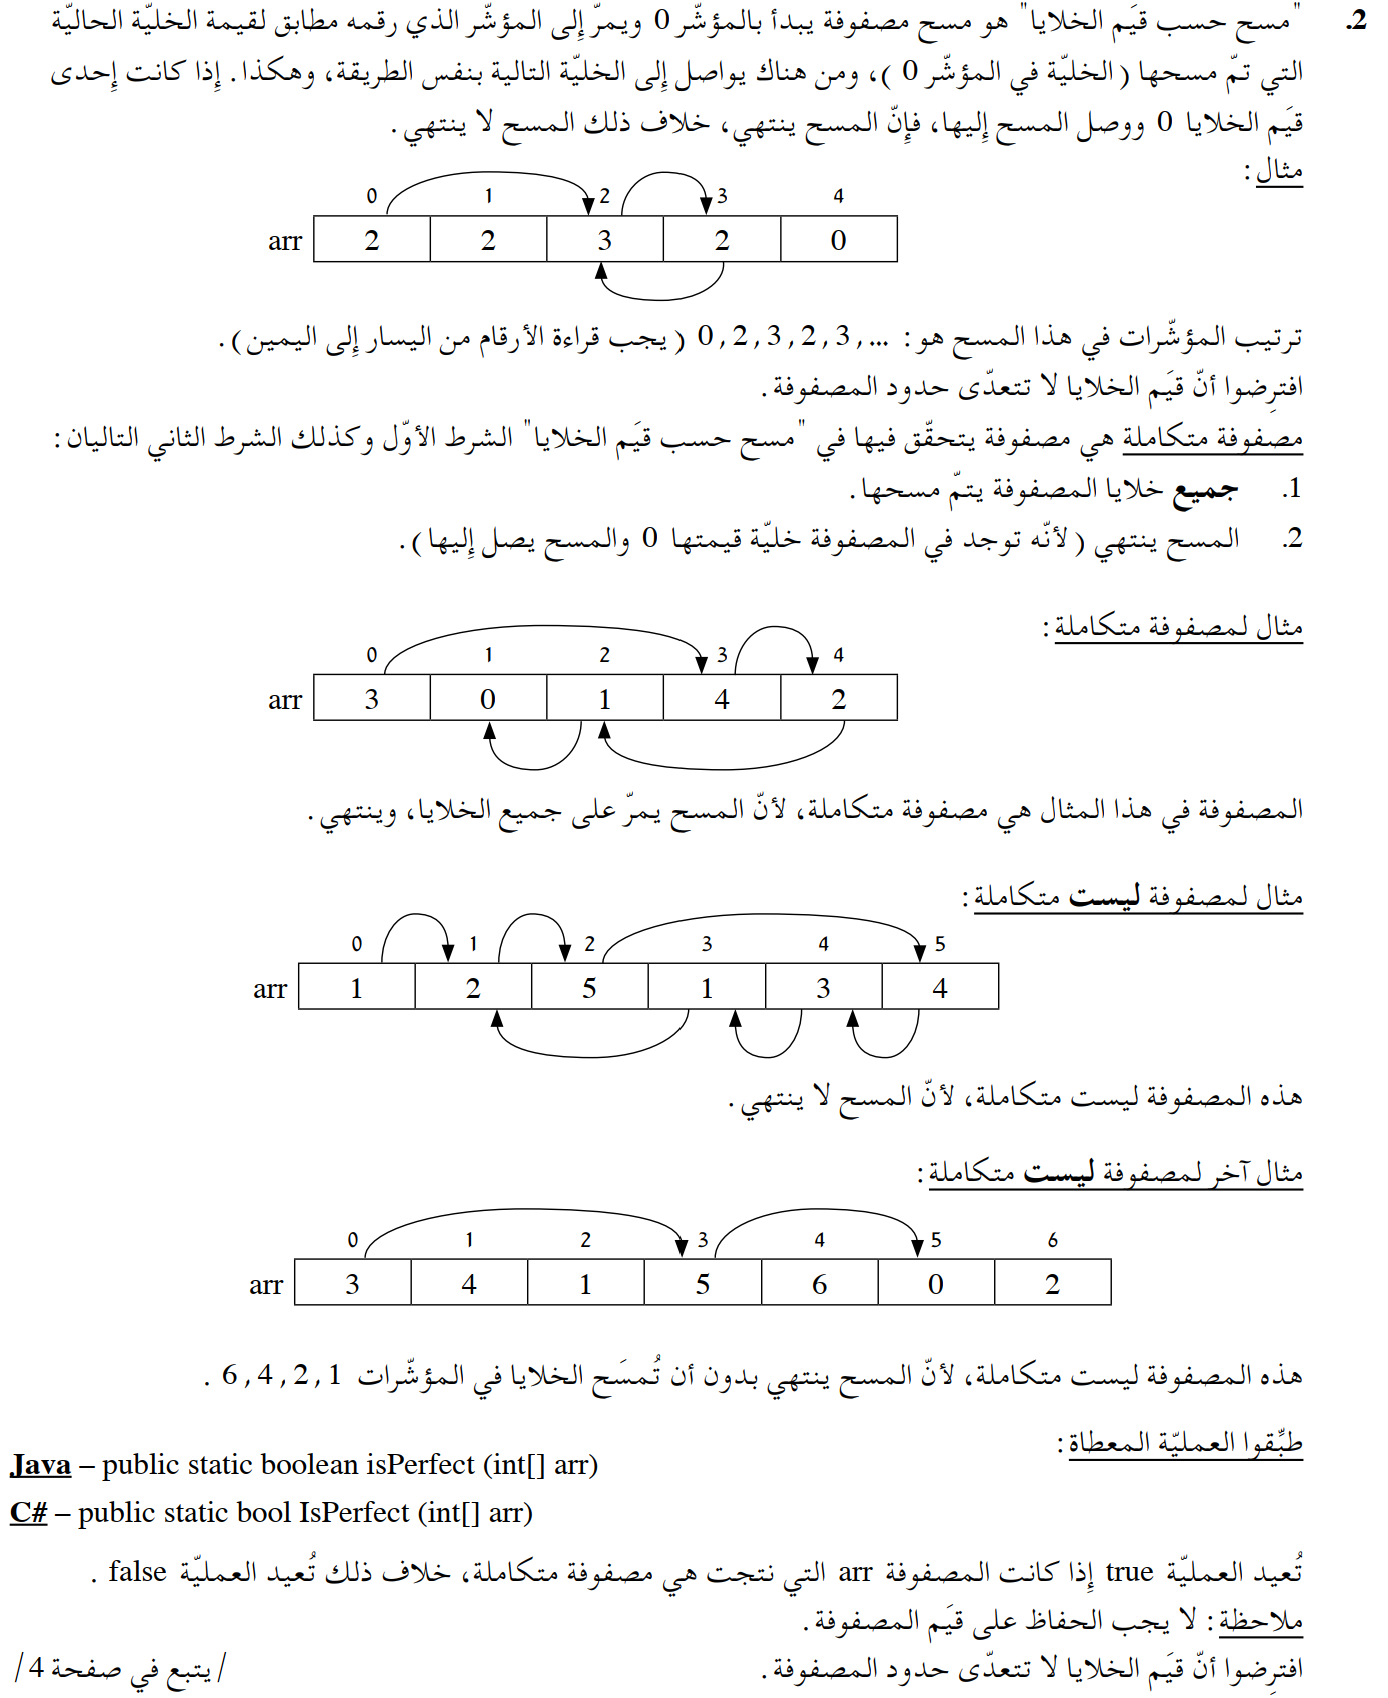
\includegraphics[width=0.8\paperwidth,keepaspectratio]{ ../../../bagrut_questions/basics/arrays_2022_899381_2.png }%
}%


\ifwithsols
\begin{boxSolution}[سؤال 2 امتحان 899381 سنة 2022]

\begin{boxCode}
\begin{english}
\begin{minted}{csharp}
static bool IsPerfect(int[] arr)
{
    int idx = arr[0];
    int tmp;
    for (int i = 0; i < arr.Length; i++)
    {
        if (arr[idx] == -1)
            return false;
        tmp = arr[idx];
        arr[idx] = -1;
        idx = tmp;
    }
    return true;
}
\end{minted}
\end{english}
\end{boxCode}

\end{boxSolution}
\clearpage
\fi

\ifwithsols
\else
\clearpage
\fi

\subsection*{سؤال 2 امتحان 899381 سنة 2023}
\addcontentsline{toc}{subsection}{سؤال 2 امتحان 899381 سنة 2023}

\noindent
\makebox[\textwidth][c]{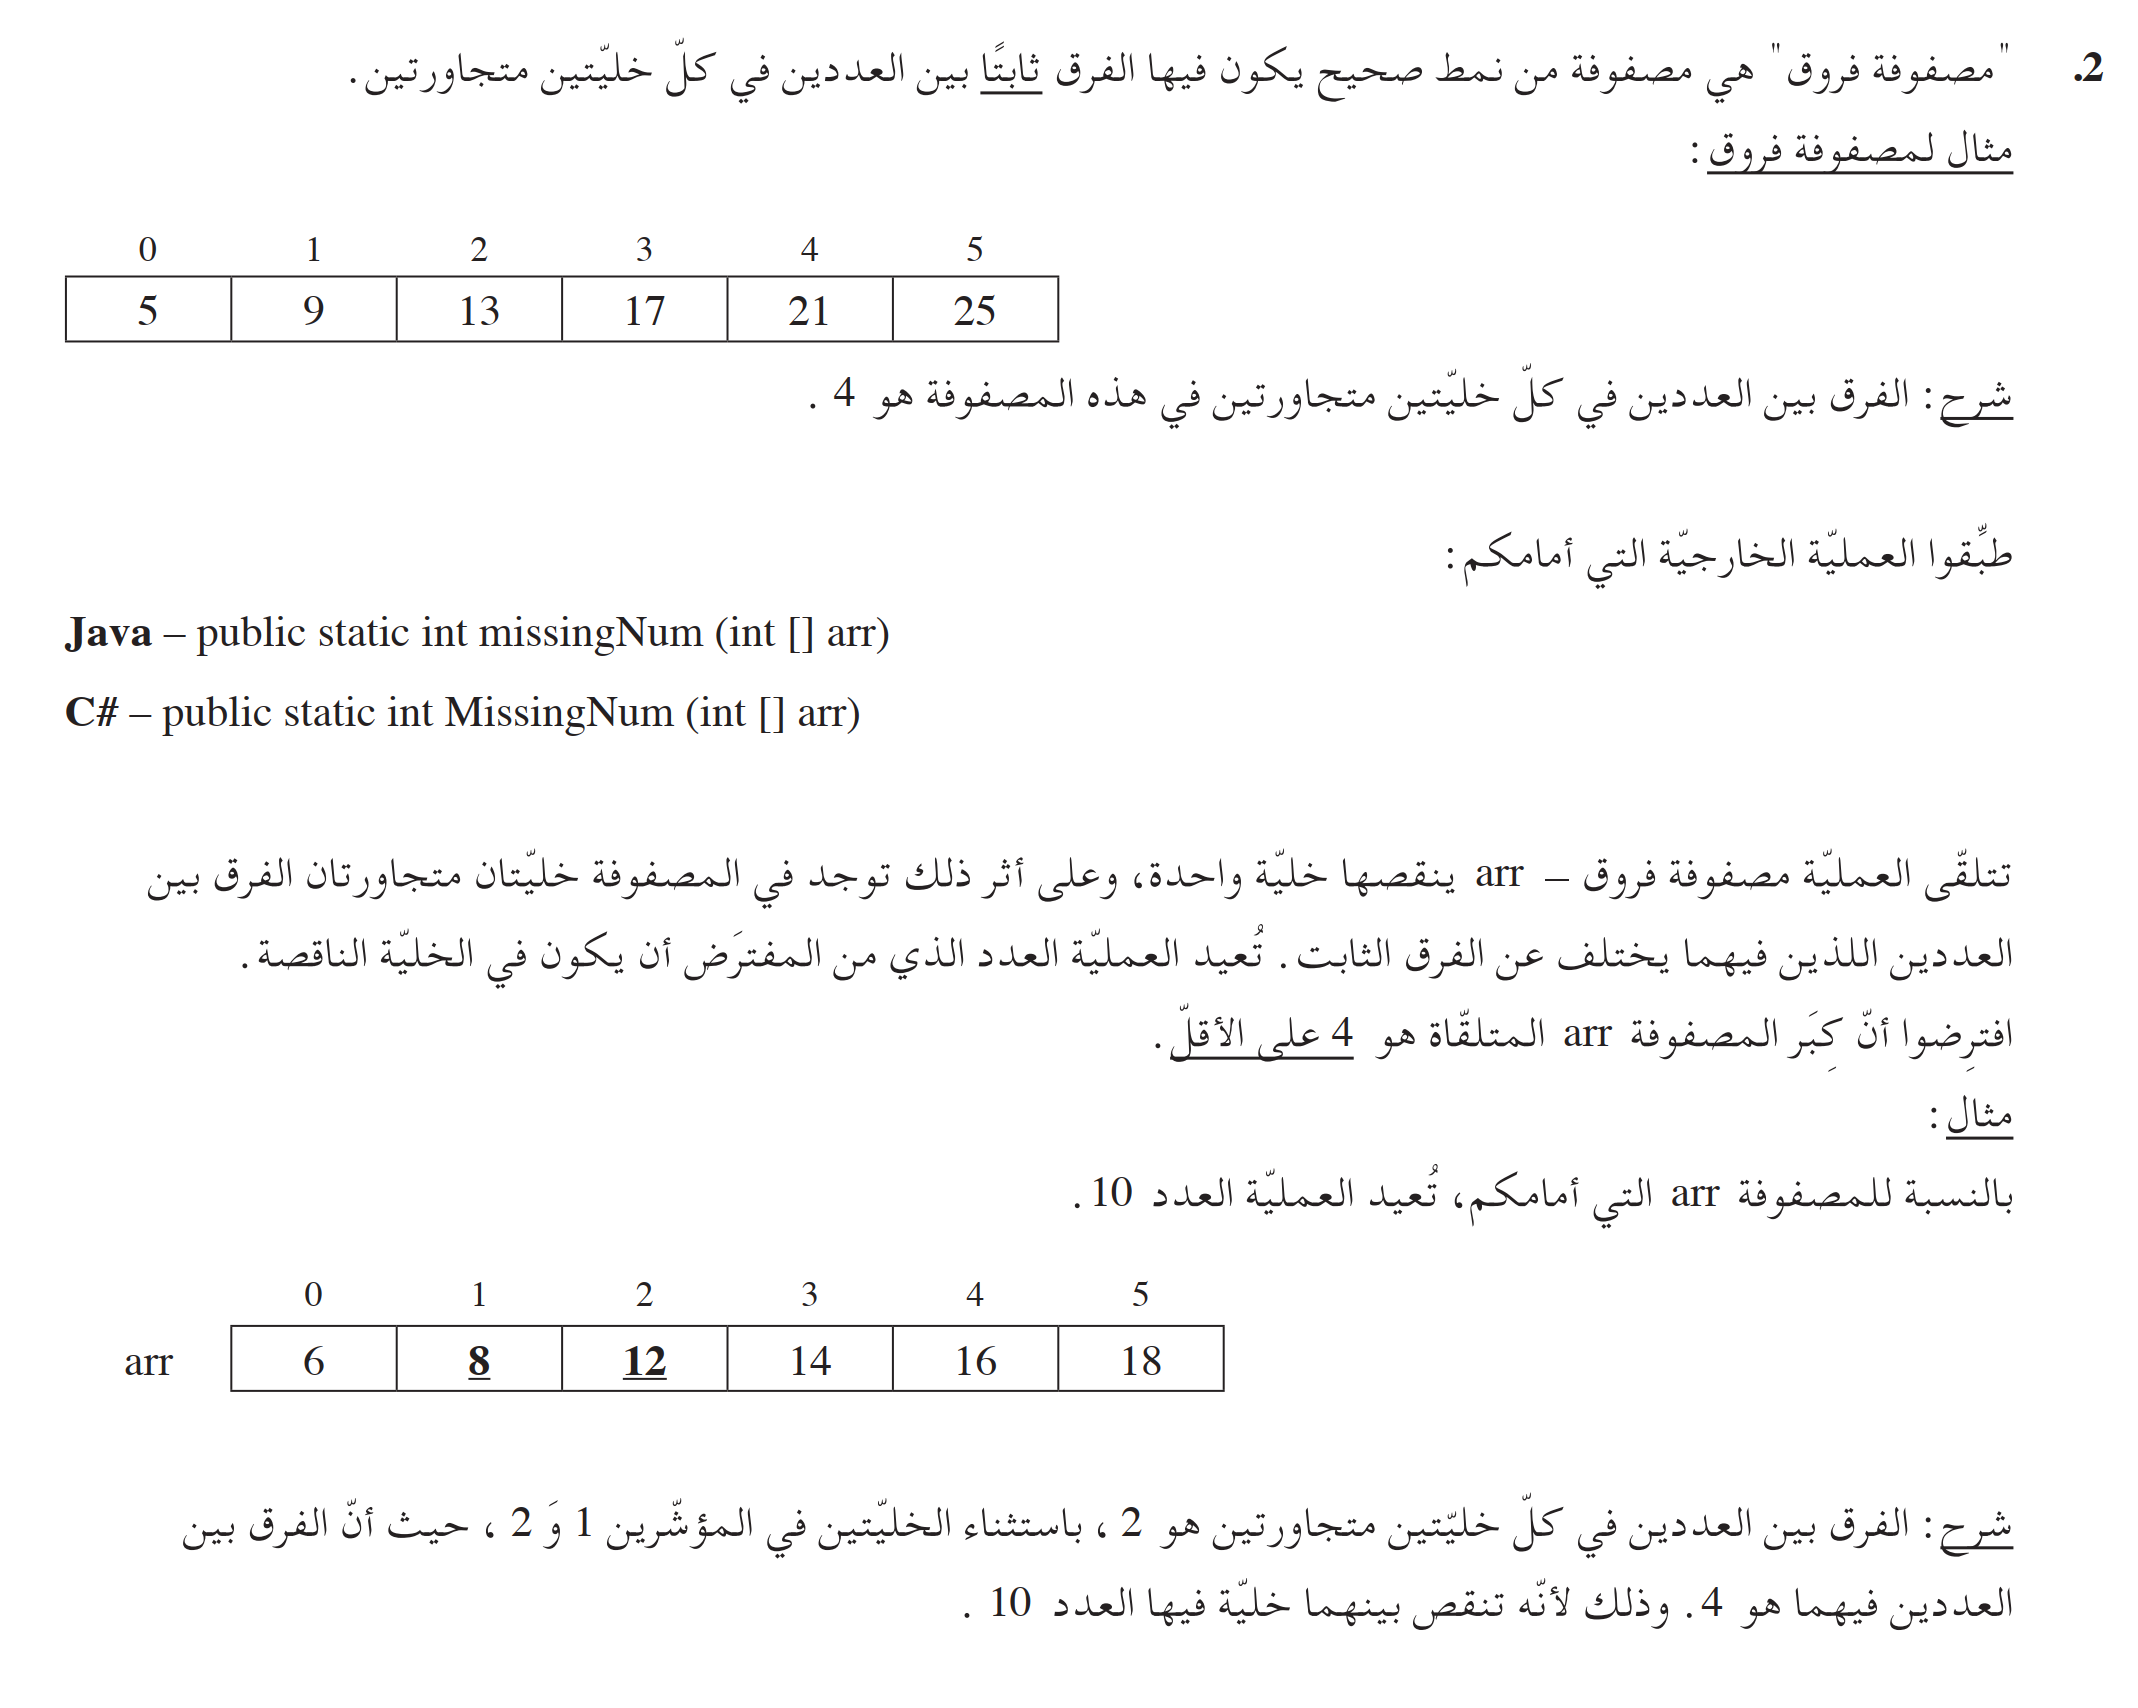
\includegraphics[width=0.9\paperwidth,keepaspectratio]{ ../../../bagrut_questions/basics/arrays_2023_899381_2.png }%
}%

\begin{boxHint}
يمكنك معرفة الفرق الثابت بين الأعداد في المصفوفة من خلال مقارنة الفرق بين أول عنصرين مع الفرق بين العنصرين الثاني والثالث. 
(الفرق الثابت هو الفرق الأصغر بينهما، أو إذا كانا متساويين فهما مساويان للفرق الثابت) \\
بعد معرفة الفرق الثابت، يمكنك المرور على المصفوفة لإيجاد العنصرين اللذين الفرقُ بينهما أكبر من الفرق الثابت، وبالتالي حساب الحد الناقص.
\end{boxHint}


\ifwithsols
\begin{boxSolution}[سؤال 2 امتحان 899381 سنة 2023]

\begin{boxCode}
\begin{english}
\begin{minted}{csharp}
public static int MissingNum(int[] arr)
{
    int diff1 = arr[1] - arr[0];
    int diff2 = arr[2] - arr[1];
    int constantDiff;
    if (diff1 <= diff2)
        constantDiff = diff1;
    else
        constantDiff = diff2;

    for (int i = 0; i < arr.Length - 1; i++)
    {
        int currentDiff = arr[i + 1] - arr[i];
        if (currentDiff != constantDiff)
            return arr[i] + constantDiff;
    }
    return -1;
}
\end{minted}
\end{english}
\end{boxCode}

\end{boxSolution}
\clearpage
\fi

\ifwithsols
\else
\clearpage
\fi

\subsection*{سؤال 2 امتحان 899371 سنة 2024}
\addcontentsline{toc}{subsection}{سؤال 2 امتحان 899371 سنة 2024}

\noindent
\makebox[\textwidth][c]{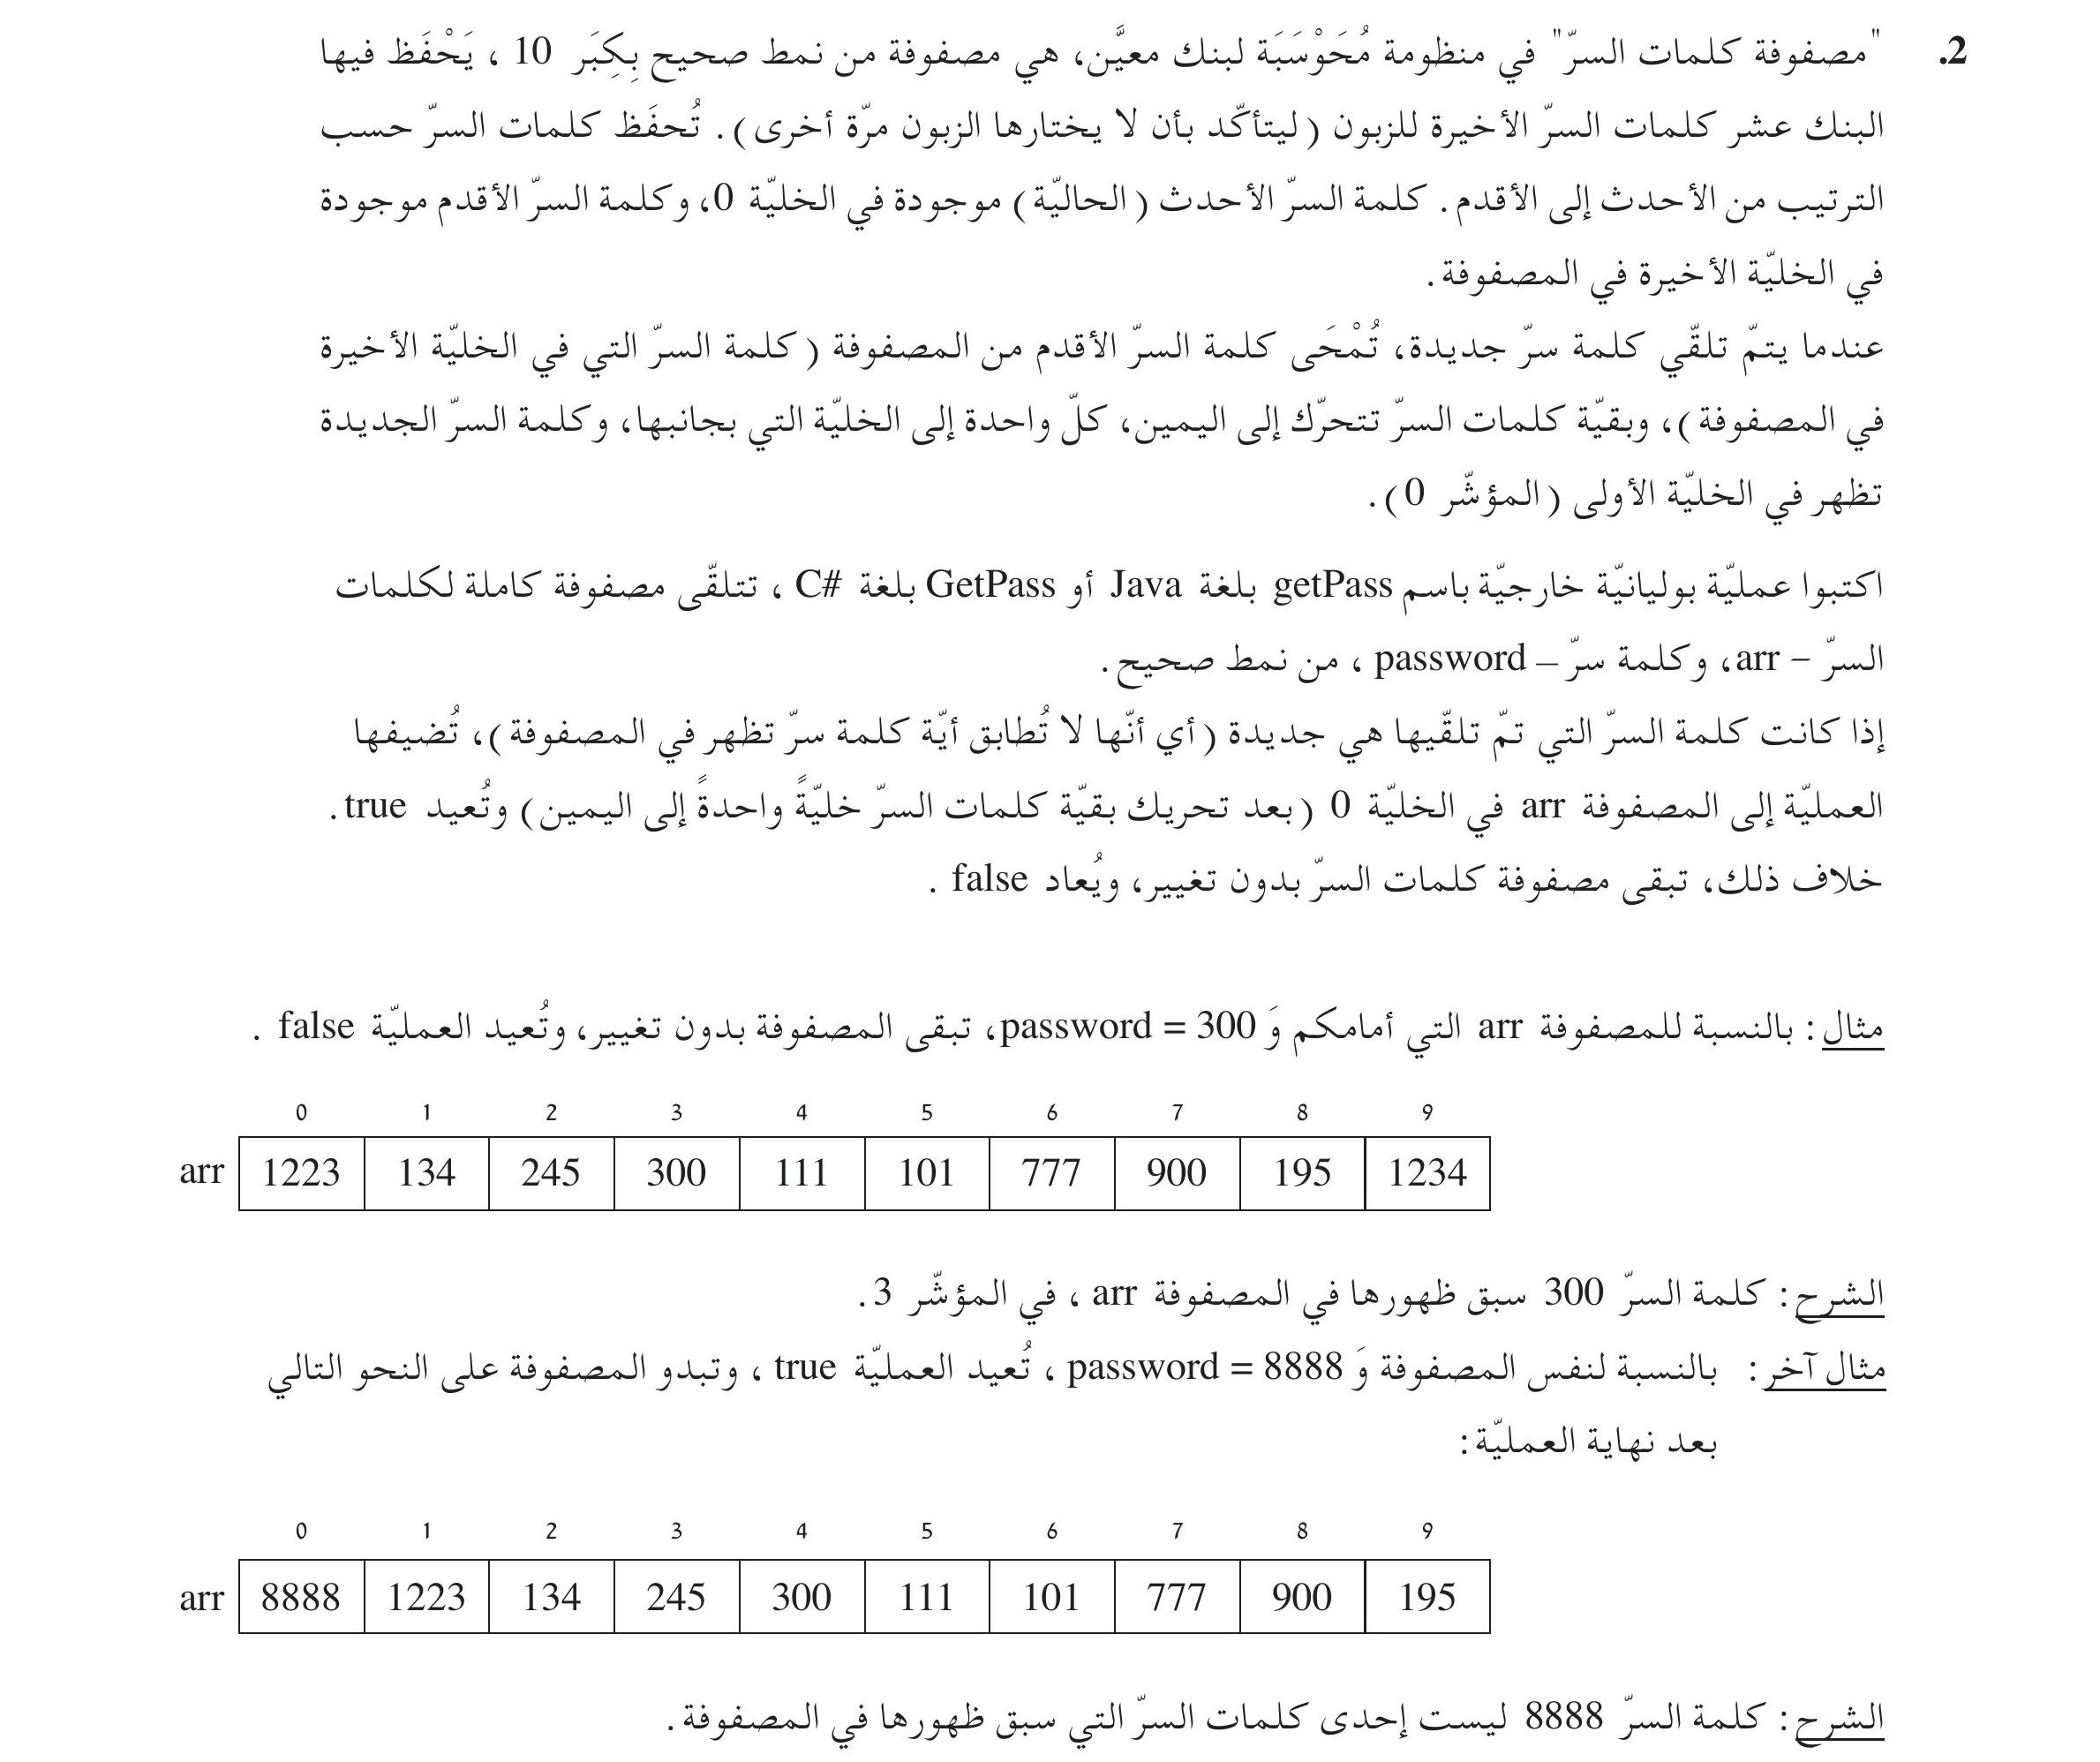
\includegraphics[width=0.9\paperwidth,keepaspectratio]{ ../../../bagrut_questions/basics/arrays_2024_899371_2.jpg }%
}%


\ifwithsols
\begin{boxSolution}[سؤال 2 امتحان 899371 سنة 2024]

\begin{boxCode}
\begin{english}
\begin{minted}{csharp}
public static bool GetPass(int[] arr, int password)
{
    // Check if password already exists in array
    for (int i = 0; i < arr.Length; i++)
    {
        if (arr[i] == password)
            return false;
    }

    // Password is new, shift all elements to the right
    for (int i = arr.Length - 1; i > 0; i--)
    {
        arr[i] = arr[i - 1];
    }
    arr[0] = password;
    return true;
}
\end{minted}
\end{english}
\end{boxCode}

\end{boxSolution}
\clearpage
\fi

\ifwithsols
\else
\clearpage
\fi

\subsection*{سؤال 2 امتحان 899371 سنة 2025}
\addcontentsline{toc}{subsection}{سؤال 2 امتحان 899371 سنة 2025}

\noindent
\makebox[\textwidth][c]{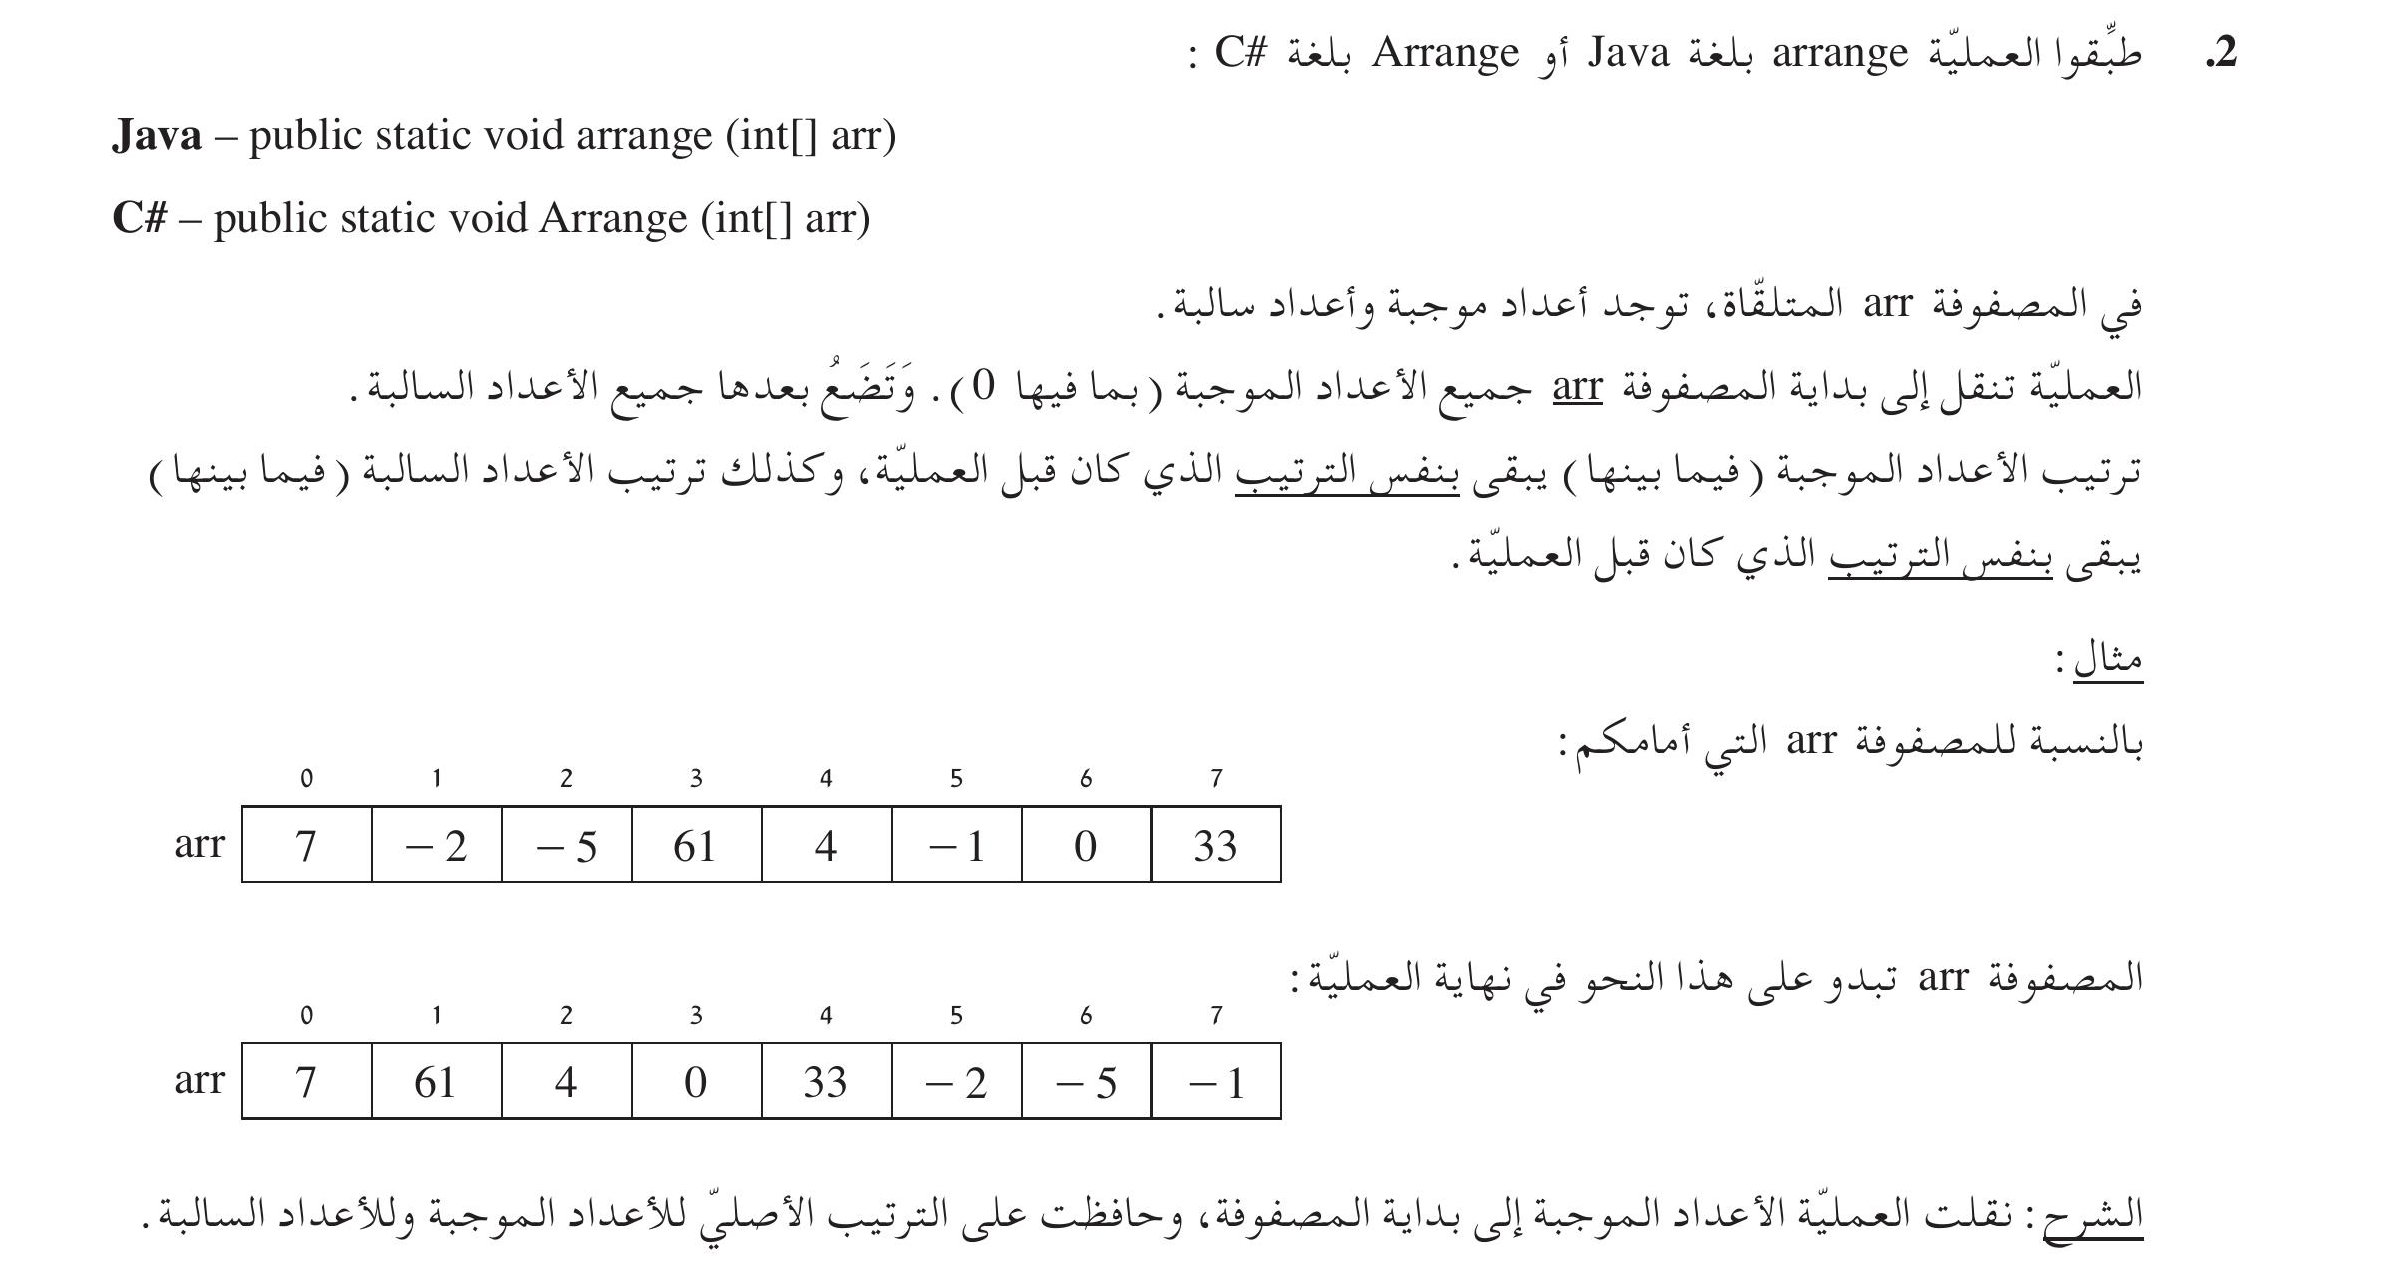
\includegraphics[width=0.9\paperwidth,keepaspectratio]{ ../../../bagrut_questions/basics/arrays_2025_899371_2.jpg }%
}%
\begin{boxHint}
    استعمل مصفوفة مساعدة، انسخ عليها أولا الأعداد الموجبة، ثم الأعداد السالبة، ثم انسخها إلى المصفوفة الأصلية.
\end{boxHint}

\ifwithsols
\begin{boxSolution}[سؤال 2 امتحان 899371 سنة 2025]
هناك عدة طرق لحل هذا السؤال:
\begin{enumerate}
    \item الطريقة الأولى: استخدام مصفوفة واحدة مساعدة
    \item الطريقة الثانية: استخدام مصفوفتين مساعدتين: واحدة لتخزين الأعداد الموجبة، والثانية للأعداد السالبة، ثم ننقلها بالترتيب إلى المصفوفة الأصلية.
    \item الطريقة الثالثة: استخدام مصفوفة واحدة لتخزين الأعداد السالبة فقط، ثم ننقل الأعداد الموجبة إلى بداية المصفوفة الأصلية، ثم ننسخ الأعداد السالبة من المصفوفة المساعدة إلى نهاية المصفوفة الأصلية.
    \item الطريقة الرابعة: بدون استخدام مصفوفة مساعدة: نبدأ من نهاية المصفوفة، في كل مرة نجد عددًا سالبًا ننسخه إلى نهاية المصفوفة (قبل الأعداد السالبة التي وجدناها حتى الآن) وننفذ إزاحة للأعداد الموجبة إلى اليسار.
\end{enumerate}
سنعرض حل الطريقة الأولى والرابعة فقط - الثانية والثالثة يمكنك كتابتها لوحدك (تشبه الطريقة الأولى).
\end{boxSolution}
\clearpage
\begin{boxSolution}[الطريقة الأولى: استخدام مصفوفة مساعدة]
{\small
\begin{itemize}
    \item في الحلقة الأولى، ننسخ جميع الأعداد الموجبة إلى مصفوفة مساعدة.
    \item في الحلقة الثانية، ننسخ جميع الأعداد السالبة إلى نفس المصفوفة المساعدة، بحيث تكون بعد الأعداد الموجبة.
    \item في الحلقة الثالثة، ننسخ العناصر من المصفوفة المساعدة إلى المصفوفة الأصلية.
\end{itemize}
}
\begin{boxCode}
\begin{english}
\begin{minted}{csharp}
public static void Arrange(int[] arr)
{
    int[] temp = new int[arr.Length];
    int index = 0;
    for (int i = 0; i < arr.Length; i++)
    {
        if (arr[i] >= 0)
        {
            temp[index] = arr[i];
            index++;
        }
    }
    for (int i = 0; i < arr.Length; i++)
    {
        if (arr[i] < 0)
        {
            temp[index] = arr[i];
            index++;
        }
    }
    for (int i = 0; i < arr.Length; i++)
    {
        arr[i] = temp[i];
    }
}
\end{minted}
\end{english}
\end{boxCode}
\end{boxSolution}

\clearpage

\begin{boxSolution}[الطريقة الرابعة: بدون استخدام مصفوفة مساعدة]
\begin{boxCode}
\begin{english}
\begin{minted}{csharp}
public static void Arrange(int[] arr)
{
    int negIdx = arr.Length - 1;
    //int nextNegIdx = arr.Length - 1;
    for (int i = arr.Length - 1; i >= 0; i--)
    {
        if (arr[i] < 0)
        {
            if (i == negIdx)
                negIdx--;
            else if (i < negIdx)
            {
                int tmp = arr[i];
                // shift all positive numbers between i and negIdx to the left
                for (int j = i; j < negIdx; j++)
                    arr[j] = arr[j + 1];
                arr[negIdx] = tmp;
                negIdx--;
            }
        }
    }
}
\end{minted}
\end{english}
\end{boxCode}

\end{boxSolution}
\clearpage
\fi

\ifwithsols
\else
\clearpage
\fi

\subsection*{سؤال 3 امتحان 899381b سنة 2020}
\addcontentsline{toc}{subsection}{سؤال 3 امتحان 899381b سنة 2020}

\noindent
\makebox[\textwidth][c]{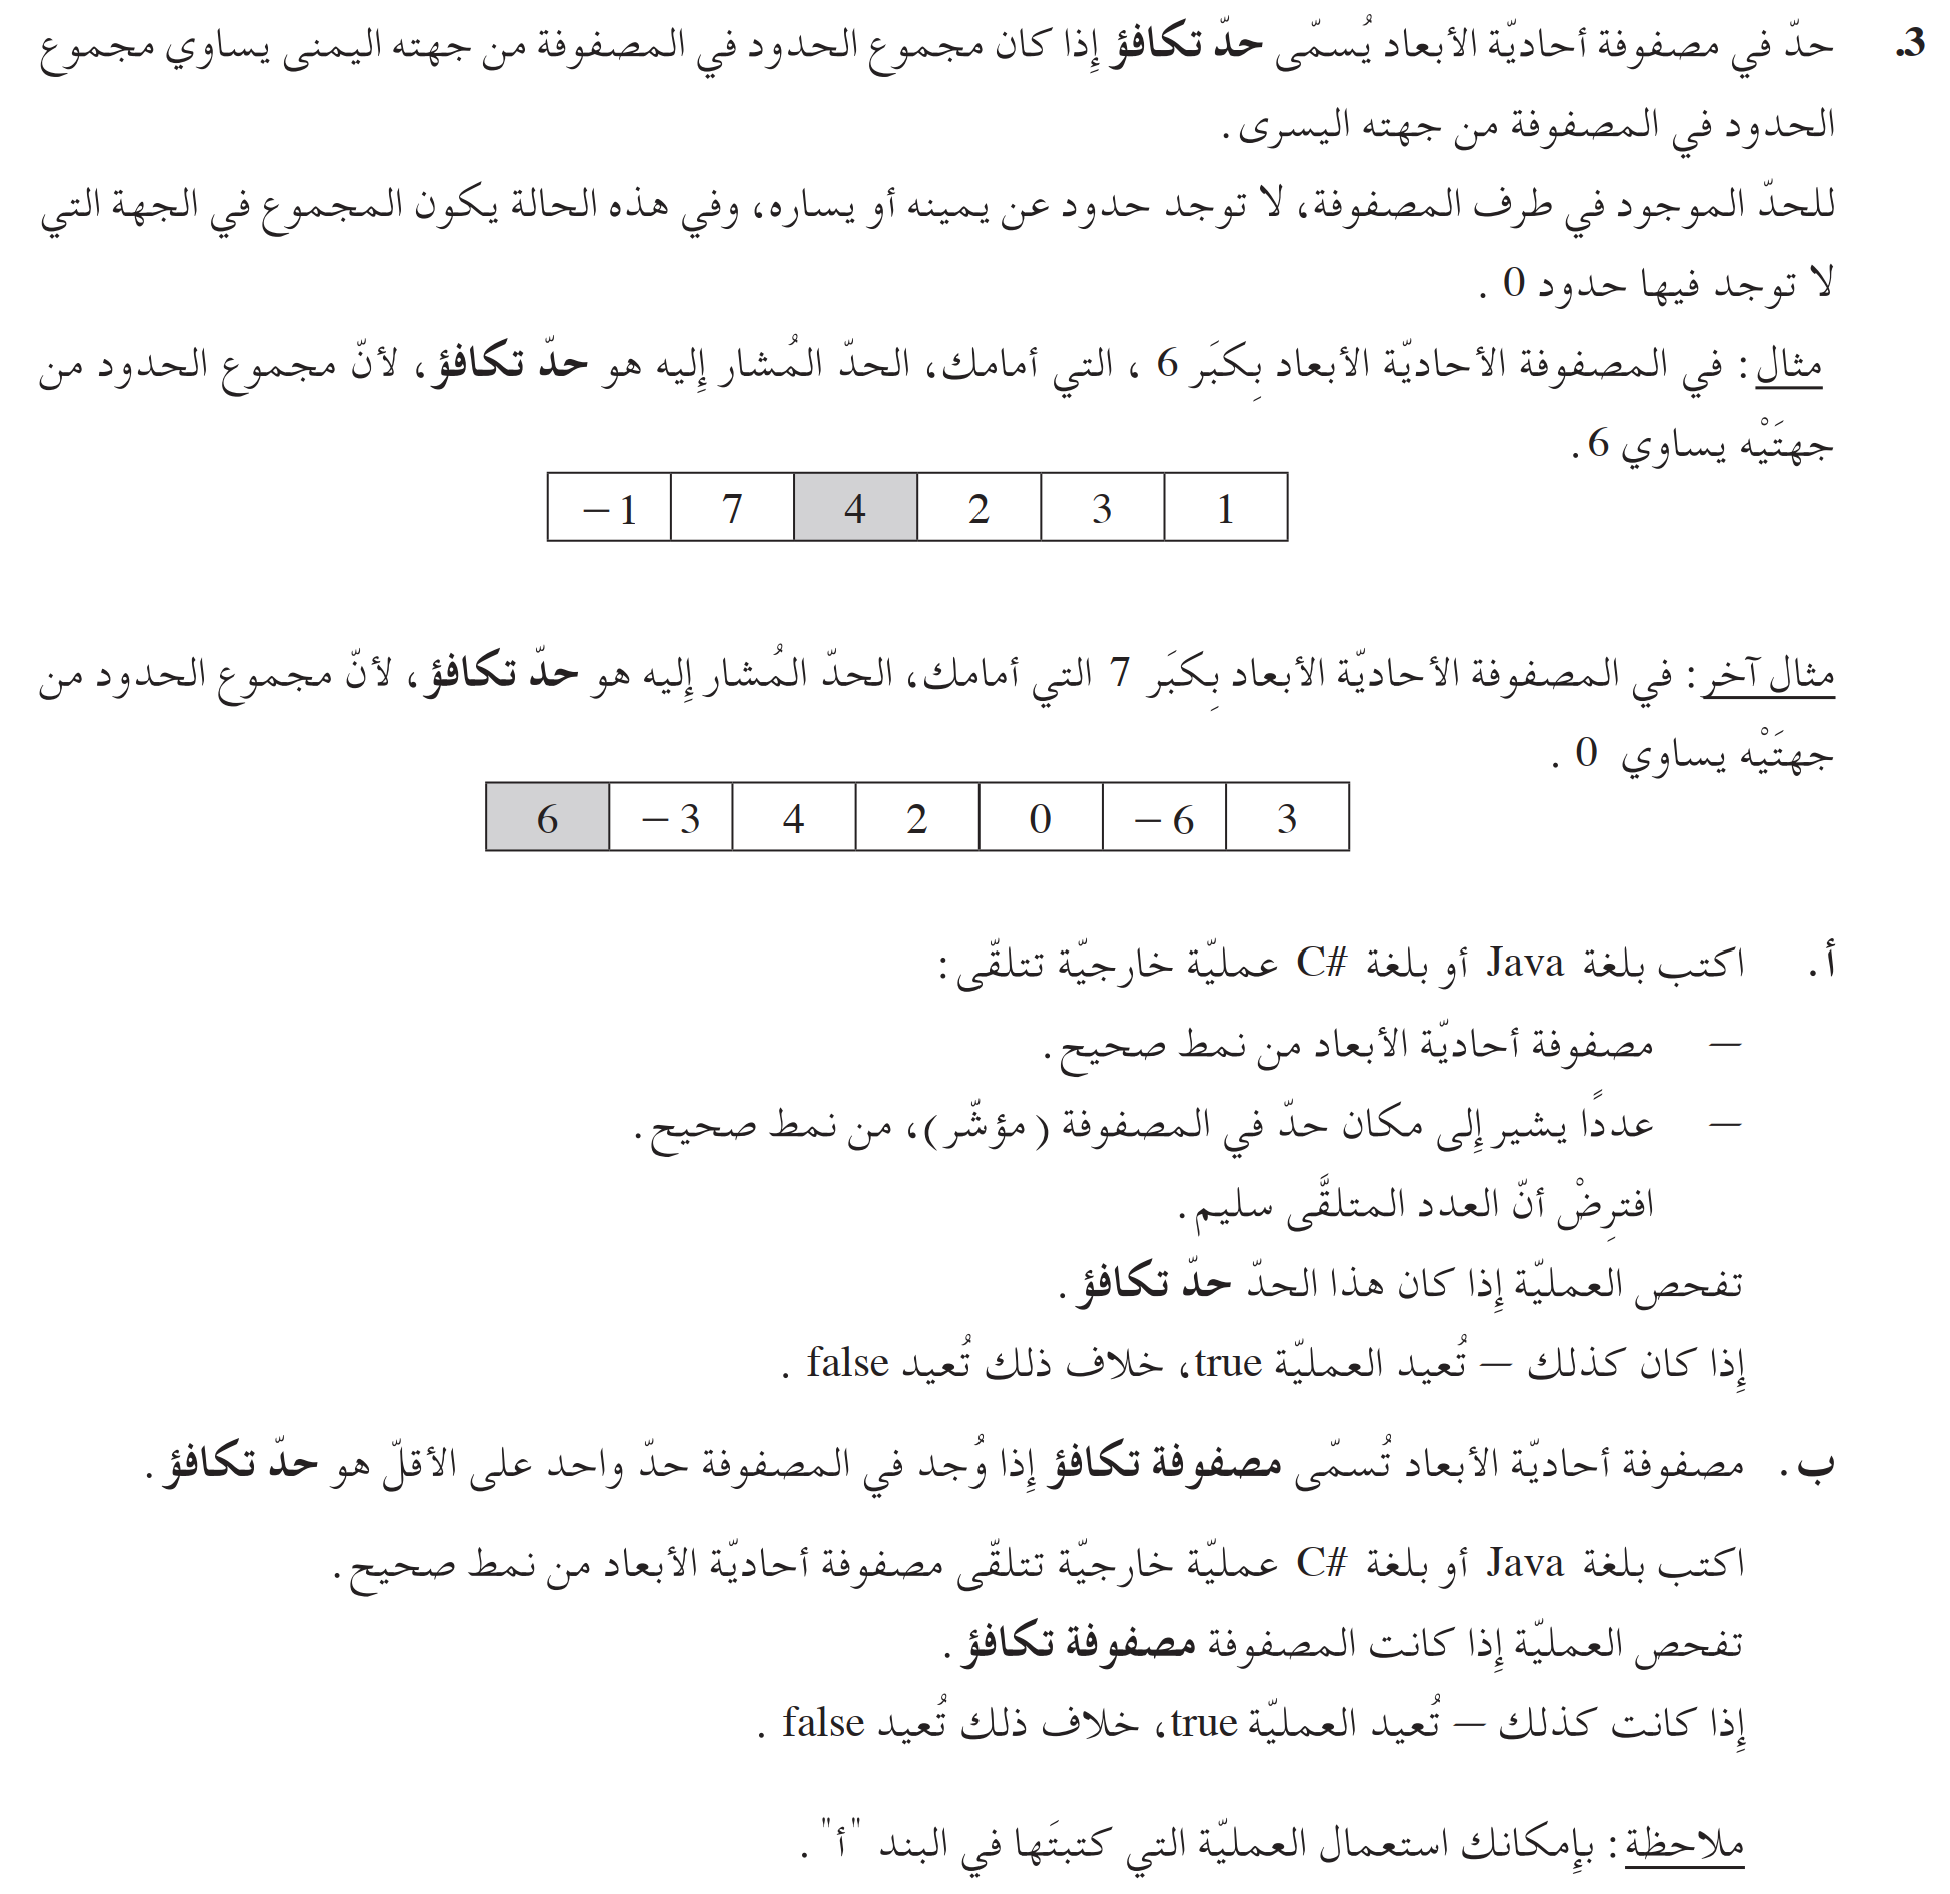
\includegraphics[width=0.9\paperwidth,keepaspectratio]{ ../../../bagrut_questions/basics/arrays_2020_899381b_3.png }%
}%


\ifwithsols
\begin{boxSolution}[سؤال 3 امتحان 899381b سنة 2020]
\begin{enumerate}[itemsep=1.5em, label=\alph*.]
    \item عملية خارجية تستقبل مصفوفة أحادية الأبعاد وعددا يشير إلى مكان حد في المصفوفة، وتفحص هذه العملية إذا كان هذا الحد حد تكافؤ.
    \item عملية خارجية تستقبل مصفوفة أحادية الأبعاد وتفحص إذا كانت المصفوفة مصفوفة تكافؤ (تحتوي على حد تكافؤ واحد على الأقل).
\end{enumerate}

\begin{boxCode}
\begin{english}
\begin{minted}{csharp}
// Part a: Check if a specific index is an equilibrium point
public static bool IsEquilibrium(int[] arr, int index)
{
    int leftSum = 0;
    int rightSum = 0;
    for (int i = 0; i < index; i++)
    {
        leftSum += arr[i];
    }
    for (int i = index + 1; i < arr.Length; i++)
    {
        rightSum += arr[i];
    }
    return leftSum == rightSum;
}

// Part b: Check if array has at least one equilibrium point
public static bool IsEquilibriumArray(int[] arr)
{
    for (int i = 0; i < arr.Length; i++)
    {
        if (IsEquilibrium(arr, i))
            return true;
    }
    return false;
}
\end{minted}
\end{english}
\end{boxCode}

\end{boxSolution}
\clearpage
\fi

\ifwithsols
\else
\clearpage
\fi

\subsection*{سؤال 3 امتحان 899371 سنة 2024}
\addcontentsline{toc}{subsection}{سؤال 3 امتحان 899371 سنة 2024}

\noindent
\makebox[\textwidth][c]{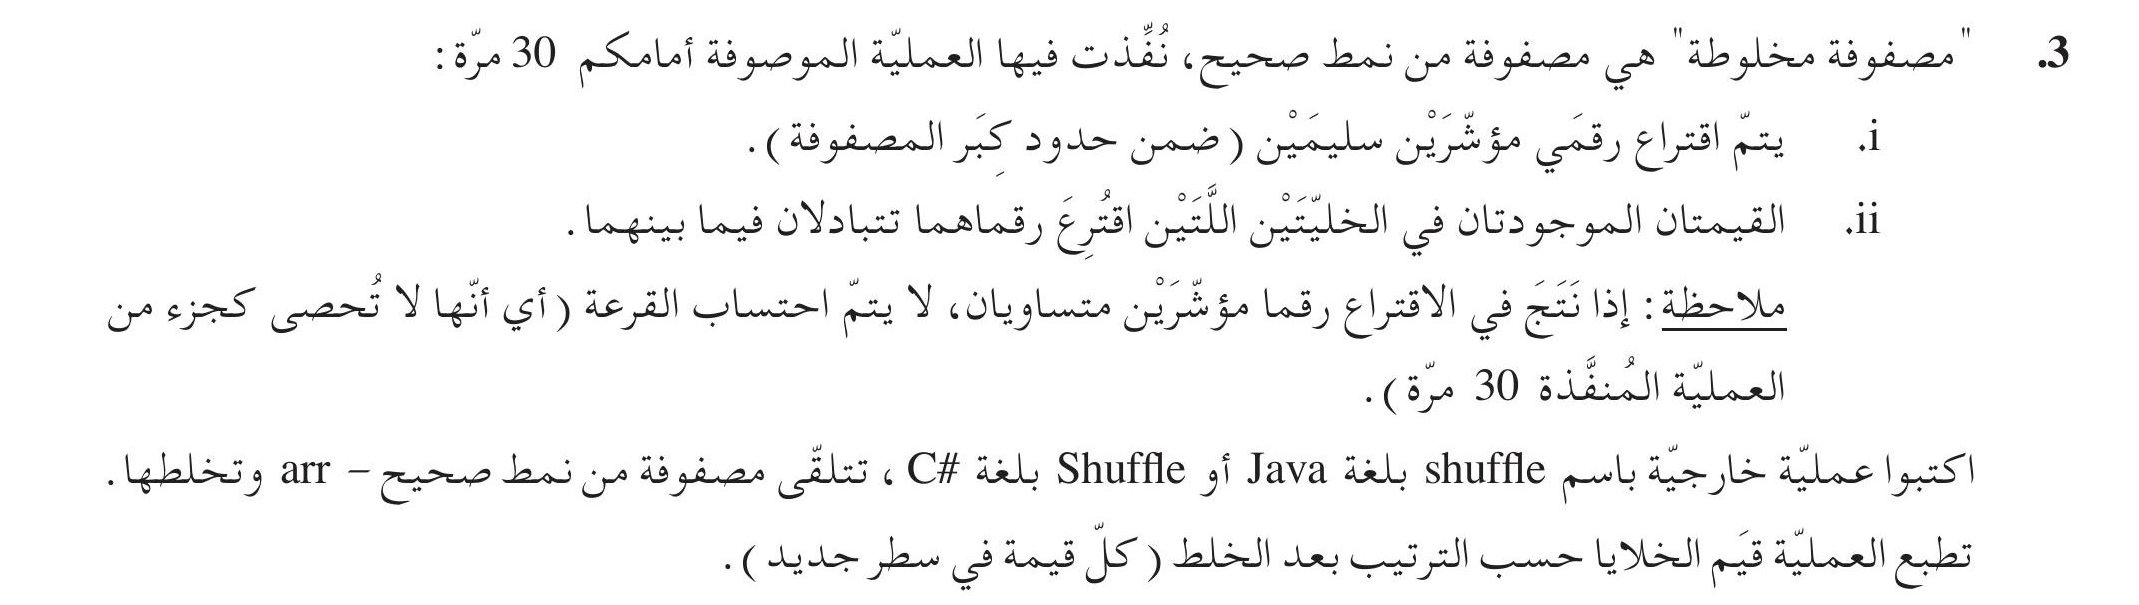
\includegraphics[width=\paperwidth,keepaspectratio]{ ../../../bagrut_questions/basics/arrays_2024_899371_3.jpg }%
}%

\begin{boxHint}
    \begin{itemize}
        \item ستحتاج إلى استخدام \texttt{Random} لتوليد أعداد عشوائية.
        \item استخدم حلقة \texttt{while}.
        \item تقديم العدّاد يحصل فقط عند نجاح عملية التبديل (أي عندما لا يكونا العنصرين المختارين نفسهما).
    \end{itemize}
\end{boxHint}

\ifwithsols
\begin{boxSolution}[سؤال 3 امتحان 899371 سنة 2024]

\begin{boxCode}
\begin{english}
\begin{minted}{csharp}
public static void Shuffle(int[] arr)
{
    Random rnd = new Random();
    int cnt = 0;
    while(cnt < 30)
    {
        int index1 = rnd.Next(arr.Length);
        int index2 = rnd.Next(arr.Length);
        if(index1 != index2)
        {
            int temp = arr[index1];
            arr[index1] = arr[index2];
            arr[index2] = temp;
            cnt++;
        }
    }
}
\end{minted}
\end{english}
\end{boxCode}

\end{boxSolution}
\clearpage
\fi

\ifwithsols
\else
\clearpage
\fi

\subsection*{سؤال 9 امتحان 899381 سنة 2022}
\addcontentsline{toc}{subsection}{سؤال 9 امتحان 899381 سنة 2022}

\noindent
\makebox[\textwidth][c]{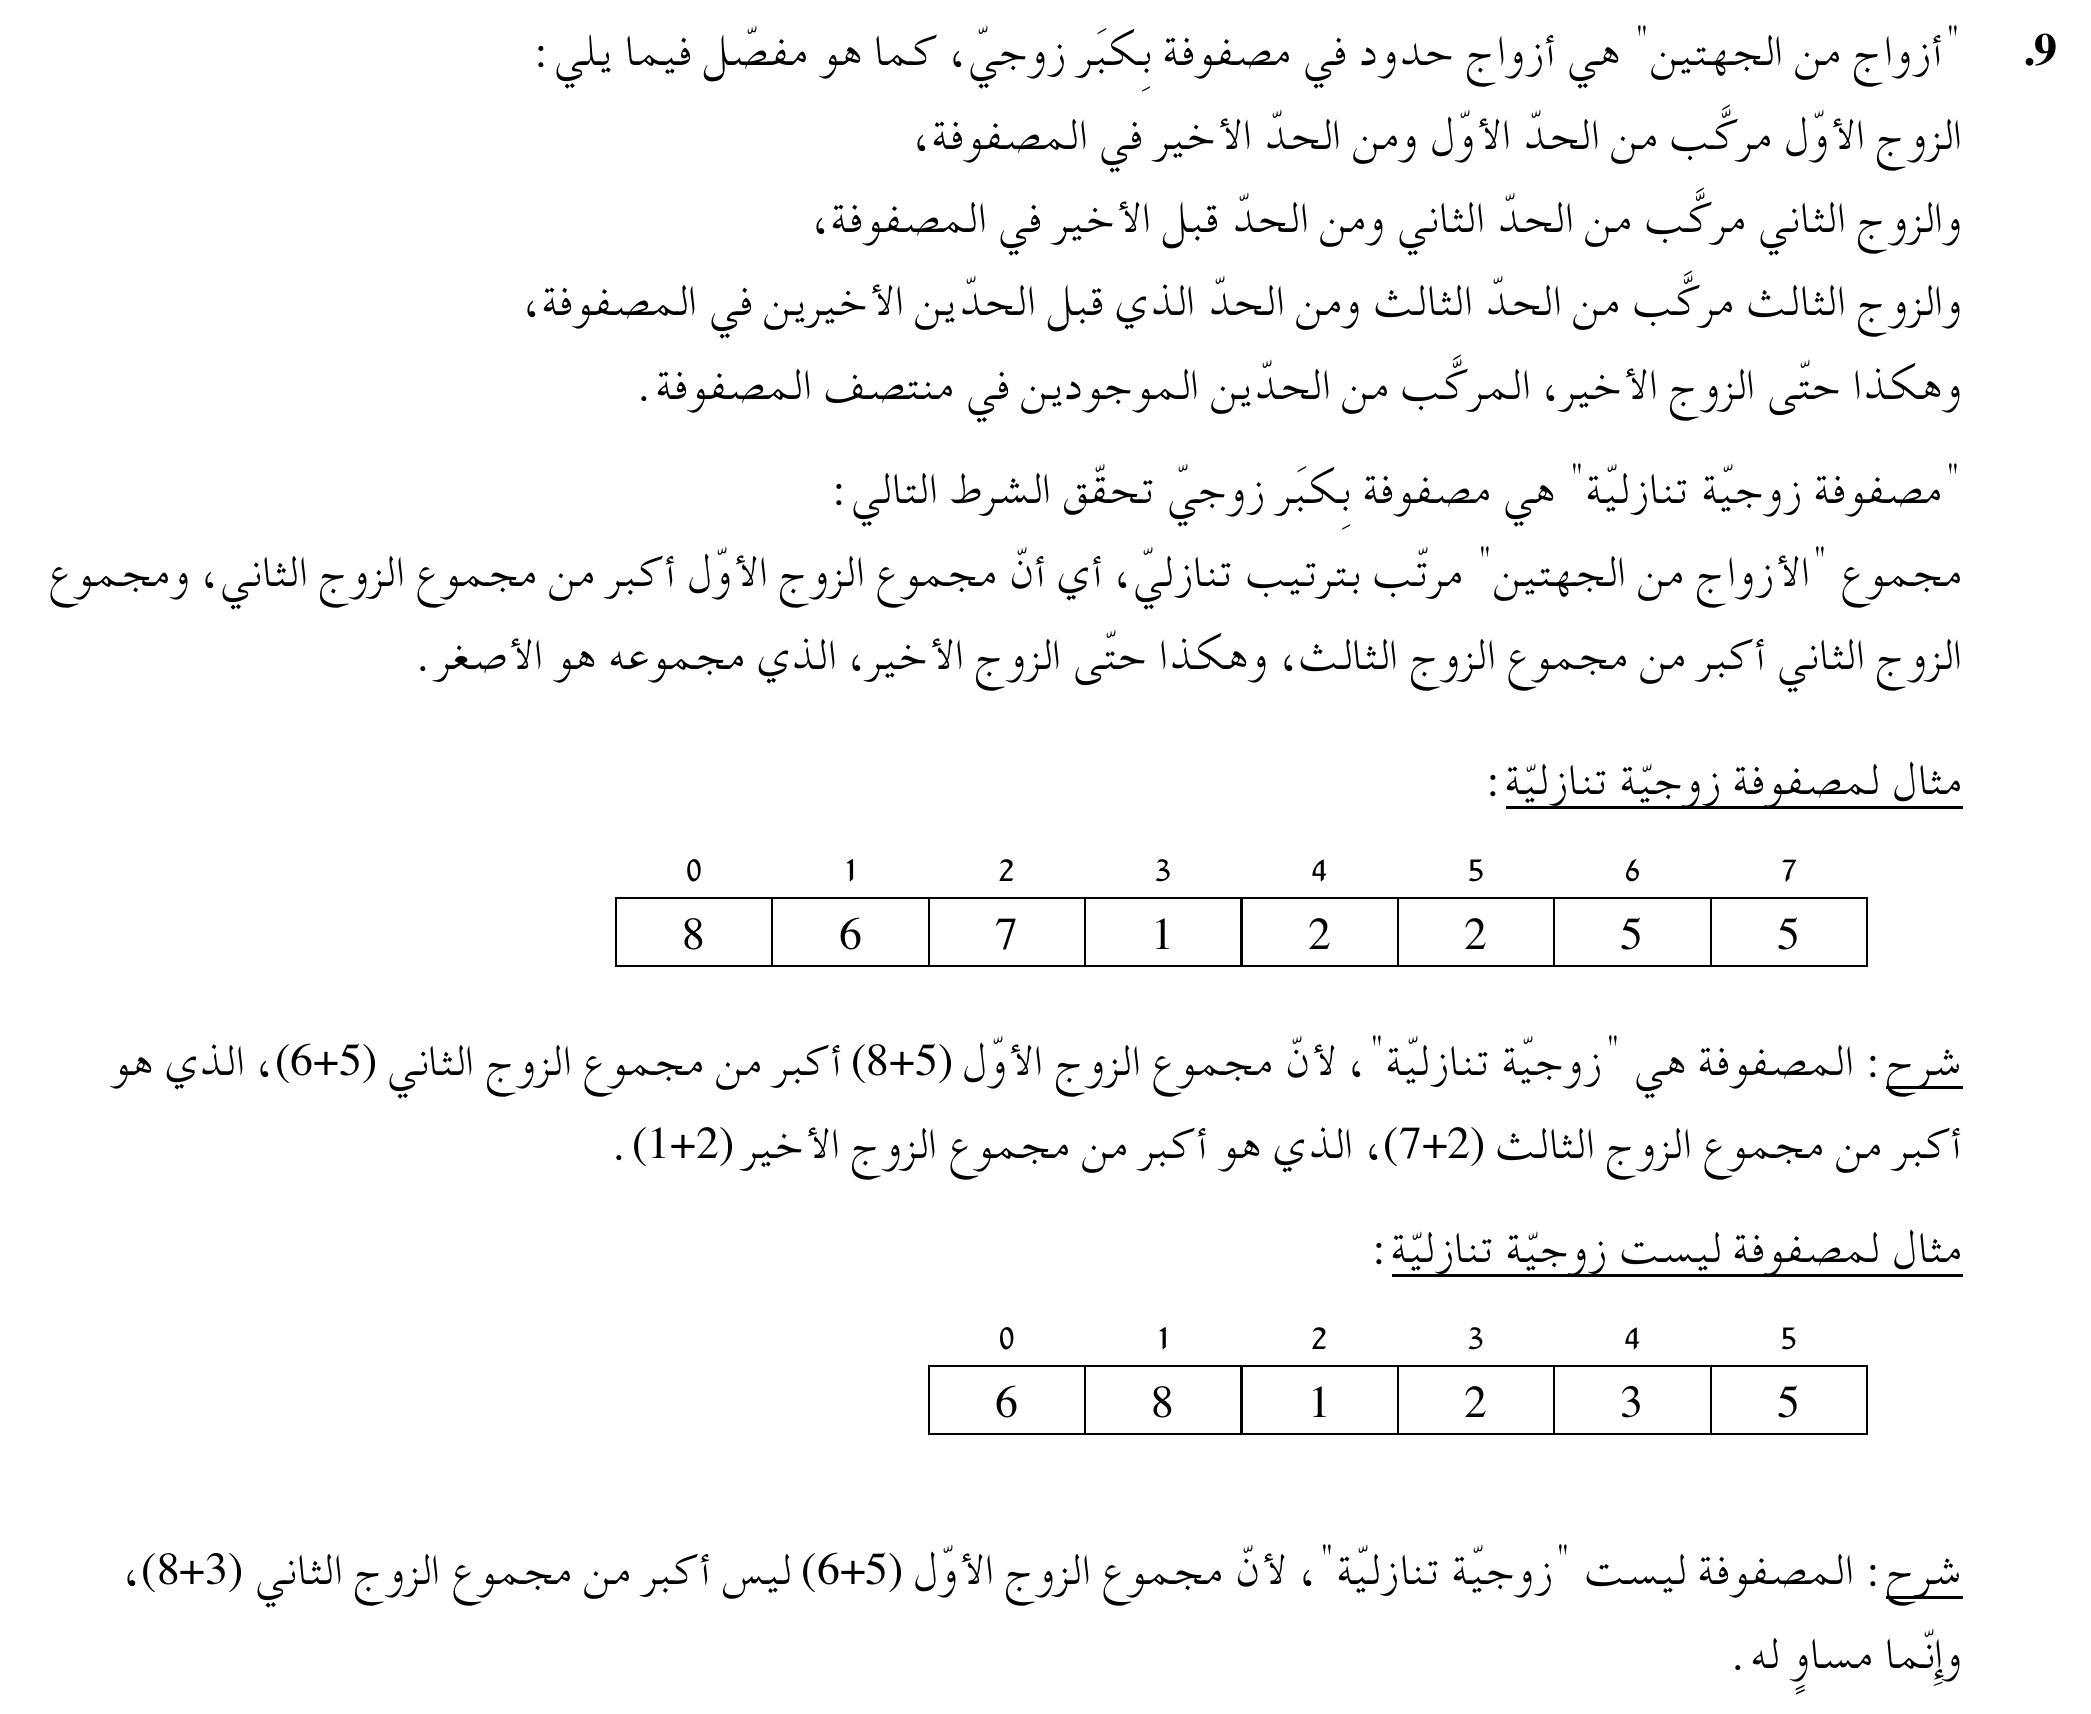
\includegraphics[width=0.9\paperwidth,keepaspectratio]{ ../../../bagrut_questions/basics/arrays_2022_899381_9.jpg }%
}%

\begin{boxHint}
    ستحتاج إلى حلقة \textenglish{for} تشبه الحلقة التي استخدمناها في سؤال \textenglish{Palindrome}، لكن بدلاً من مقارنة العناصر المتقابلة، ستقوم بجمعها ثم تقارن...
\end{boxHint}

\ifwithsols
\begin{boxSolution}[سؤال 9 امتحان 899381 سنة 2022]

\begin{boxCode}
\begin{english}
\begin{minted}{csharp}
public static bool IsDescendingPairs(int[] arr)
{
    int prevPairSum = arr[0] + arr[arr.Length - 1];
    int currentPairSum;
    for (int i = 1; i < arr.Length / 2 - 1; i++)
    {
        currentPairSum = arr[i] + arr[arr.Length - 1 - i];
        if (currentPairSum <= prevPairSum)
            return false;
        prevPairSum = currentPairSum;
    }
    return true;
}
\end{minted}
\end{english}
\end{boxCode}

\end{boxSolution}
\clearpage
\fi


\end{document}
